%% Package and Class "uiucthesis2014" for use with LaTeX2e.
\documentclass[edeposit,fullpage]{uiucthesis2018}


\usepackage[acronym,toc]{glossaries}
\newacronym{cta}{CTA}{Chicago Transit Authority}
\newacronym{usa}{USA}{United States of America}
\newacronym{ceja}{CEJA}{Climate and Equitable Jobs Act}
\newacronym{padd}{PADD}{Petroleum Administration for Defense District}
\newacronym{smr}{SMR}{Steam Methane Reformation}
\newacronym{hds}{HDS}{hydrodesulfurization}
\newacronym{esom}{ESOM}{Energy System Optimization Model}
\newacronym{hgl}{HGL}{hydrocarbon gas liquids}
\newacronym{btu}{Btu}{British thermal unit}
\newacronym{eia}{EIA}{U.S. Energy Information Administration}
\newacronym{swu}{SWU}{separative work units}
\newacronym{triso}{TRISO}{TRi-structural ISOtropic}
\newacronym{uf}{UF}{Used Fuel}
\newacronym{nfc}{NFC}{nuclear fuel cycle}
\newacronym{lwr}{LWR}{Light Water Reactor}
\newacronym{ipyc}{IPyC}{Inner PyroCarbon layer}
\newacronym{opyc}{OPyC}{Outer PyroCarbon layer}
\newacronym{htgr}{HTGR}{High-Temperature Gas-cooled Reactor}
\newacronym{uk}{UK}{United Kingdom}
\newacronym{fb-cvd}{FB-CVD}{Fluidized-Bed Chemical Vapor Deposition system}
\newacronym{bwxt}{BWXT}{BWX Technologies, Inc.}
\newacronym{usnc}{USNC}{Ultra Safe Nuclear Corporation}
\newacronym{nrc}{NRC}{U.S. Nuclear Regulatory Commission}
\newacronym{pfm}{PFM}{the Pilot Fuel Manufacturing facility}
\newacronym{tf3}{TF3}{the TRISO-X Fuel Fabrication Facility}
\newacronym{wna}{WNA}{the World Nuclear Association}
\newacronym{bwr}{BWR}{Boiling Water Reactor}
\newacronym{pwr}{PWR}{Pressurized Water Reactor}
\newacronym{hwr}{HWR}{Heavy Water Reactor}
\newacronym{gcr}{GCR}{Gas Cooled Reactor}
\newacronym{msr}{MSR}{Molten Salt Reactor}
\newacronym{lmfbr}{LMFBR}{Liquid Metal Fast Breeder Reactor}
\newacronym{rmbk}{RMBK}{graphite-moderated water-cooled reactor}
\newacronym{tru}{TRU}{transuranic isotopes}
\newacronym{mox}{MOX}{mixed oxide fuel}
\newacronym{leu+}{LEU$^+$}{low enriched uranium$^+$}
\newacronym{haleu}{HALEU}{high assay low enriched uranium}
\newacronym{dre}{DRE}{Dynamic Resource Exchange}
\newacronym{ever}{EVER}{Enrichment Versatile non-Equilibrium Reactor}
\newacronym{clover}{CLOVER}{Core LOading versatile non-Equilibrium Reactor}
\newacronym{doe}{DOE}{U.S. Department of Energy}
\newacronym{pris}{PRIS}{Power Reactor Information System}
\newacronym{iaea}{IAEA}{International Atomic Energy Agency}
\newacronym{arfc}{ARFC}{Advanced Reactors and Fuel Cycles}
\newacronym{ercot}{ERCOT}{Electric Reliability Council of Texas}
\newacronym{esm}{ESM}{Energy System Model}
\newacronym{iea}{IEA}{International Energy Agency}
\newacronym{iiasa}{IIASA}{International Institute for Applied Systems Analysis}
\newacronym{bau}{BAU}{Business-as-Usual}
\newacronym{leu}{LEU}{low enriched uranium}
\newacronym{heu}{HEU}{highly enriched uranium}
\newacronym{nea}{NEA}{Nuclear Energy Agency}
\newacronym{fbcvd}{FB-CVD}{fluidized-bed chemical vapor deposition system}
\newacronym{aec}{AEC}{Atomic Energy Commission}
\newacronym{mmr}{MMR}{Micro Modular Reactor}
\newacronym{fhr}{FHR}{Fluoride Salt-Cooled, High Temperature Reactor}

\usepackage{xspace}
\usepackage{graphics}
\newcommand{\cycamore}{\textsc{Cycamore}\xspace}
\newcommand{\cyclus}{\textsc{Cyclus}\xspace}

\usepackage{longtable}
\usepackage[section]{placeins}
\usepackage{booktabs} % nice rules (thick lines) for tables
\usepackage{microtype} % improves typography for PDF
\usepackage{float}
\usepackage[hyphens]{url}
\usepackage{hyperref}
\hypersetup{hidelinks}
\usepackage{subfig}
\usepackage{hhline}
\usepackage{amsmath}
\usepackage{array}
\usepackage{color}
\usepackage{multirow}
\usepackage{siunitx}
\sisetup{
    input-decimal-markers = .,input-ignore = {,},table-number-alignment = right,
    group-separator={,}, group-four-digits = true
}
\usepackage{fourier}
\usepackage{booktabs}
\newcommand\tab[1][1cm]{\hspace*{#1}}

\newcommand{\RomanNumeralCaps}[1]
    {\MakeUppercase{\romannumeral #1}}

\usepackage{threeparttable, tablefootnote}

%tikzpicture fit to page width
\usepackage{environ}
\makeatletter
\newsavebox{\measure@tikzpicture}
\NewEnviron{scaletikzpicturetowidth}[1]{%
  \def\tikz@width{#1}%
  \def\tikzscale{1}\begin{lrbox}{\measure@tikzpicture}%
  \BODY
  \end{lrbox}
  \pgfmathparse{#1/\wd\measure@tikzpicture}%
  \edef\tikzscale{\pgfmathresult}%
  \BODY
}

\usepackage{tabularx}
\newcolumntype{b}{>{\hsize=1.0\hsize}X}
\newcolumntype{q}{>{\hsize=0.5\hsize}X}
\newcolumntype{R}{>{\raggedleft\arraybackslash\hsize=0.5\hsize}X}
\newcolumntype{z}{>{\hsize=0.75\hsize}X}
% \newcolumntype{s}{>{\hsize=.5\hsize}X}
\newcolumntype{m}{>{\hsize=.75\hsize}X}

\usepackage{cleveref}
\usepackage{datatool}
\usepackage[numbers]{natbib}
\usepackage{notoccite}


\usepackage{tikz}
\usetikzlibrary{positioning, arrows, decorations, shapes, angles, quotes}

\tikzstyle{line} = [draw, -latex']

\definecolor{lightpurple}{HTML}{ECD9ED}
\definecolor{lightgreen}{HTML}{CAE0AB}
\definecolor{lightblue}{HTML}{6D9EEB}


\tikzstyle{block} = [rectangle, draw, fill=lightgreen!20,
    text width=8em, text centered, rounded corners, minimum height=4em]

  \tikzstyle{blockfront} = [rectangle, draw, fill=lightgreen!20,
    text width=7em, text centered, rounded corners, minimum height=4em]
\tikzstyle{blockreactor} = [rectangle, draw, fill=lightblue!20,
    text width=7em, text centered, rounded corners, minimum height=4em]
\tikzstyle{blockback} = [rectangle, draw, fill=lightpurple!20,
    text width=7em, text centered, rounded corners, minimum height=4em]

\tikzstyle{abc} = [rectangle, draw, fill=lightgreen!20, text width=6em, text
    centered, rounded corners, minimum height=4em]

\title{LEU+ to HALEU nuclear fuel cycle transitions and Dynamic Reactor Models}

% Dynamic Reactor Models and LEU+ to HALEU transitions in nuclear fuel cycles
% LEU+ to HALEU transitions in nuclear fuel cycles
% LEU+ to HALEU transitions in advanced reactor fuel cycles
% Dynamic Modeling of Advanced Reactor Fuel Cycles and LEU+ to HALEU
\author{Nathan Sean Ryan}
\department{Nuclear, Plasma, Radiological Engineering}
\schools{B.S., University of Illinois - Urbana Champaign, 2022}
\msthesis
\advisor{Madicken Munk}
\degreeyear{2025}
\committee{Assistant Professor Madicken Munk \\ Associate Professor Kathryn D. Huff \\ Professor Rizwan Uddin}

\begin{document}
\maketitle

\frontmatter
%% Create an abstract that can also be used for the ProQuest abstract.
%% Note that ProQuest truncates their abstracts at 350 words.
\begin{abstract}

%% Create an abstract that can also be used for the ProQuest abstract.
%% Note that ProQuest truncates their abstracts at 350 words.
This is the abstract.



\textbf{Keywords:} Cyclus, TRISO, Nuclear Fuel Cycle, Memory Efficiency
\glsresetall

\end{abstract}

\chapter*{Acknowledgments}

I would like to thank Prof. Madicken Munk, who introduced me into
the nuclear community as a newly minted graduate student and who inspires
constantly with her intelligence and warmth. Relatedly, I would like to thank
Prof. Kathryn Huff, who has been a mentor and advisor to me at every step of my
collegiate education and who guided me in the home stretch of this work.

I would like to thank my fellow graduate students and the members of
\gls{arfc} especially Amanda Bachmann, Sam Dotson, Nataly Panczyk, Olek Yardas,
Zo\"{e} Richter, Luke Seifert, Gwendolyn Chee, Sun Myung Park, Rhys MacMillian,
and Ceser Zambrano.

Throughout the years, I learned much from my group mates, advisors, and
mentors, but I would be remiss to not acknowledge that I went to the school of
open source and learned much from countless developers who work openly to
better science. In particular the \cyclus community, especially Prof. Paul P.H.
Wilson, Jin Whan Bae, and Dr. Eva Davidson.

I owe many thanks to my parents, brother, grandparents, family, partner, and
friends who have reminded me--sometimes to my chagrin--that life keeps going
outside the walls of my office. To my cousin Matthew, I can not wait to explain
this part of my life to you someday when we are reunited because I know you are
going to have questions.

This research is being performed using funding received from the DOE Office of
Nuclear Energy's Nuclear Energy University Program (Project 23-29656
DE-NE0009390) 'Illuminating Emerging Supply Chain and Waste Management
Challenges'.

This research was supported in part by an appointment to the Oak Ridge National
Laboratory Research Student Internships Program, sponsored by the U.S.
Department of Energy and administered by the Oak Ridge Institute for Science
and Education.

%% The thesis format requires the Table of Contents to come
%% before any other major sections, all of these sections after
%% the Table of Contents must be listed therein (i.e., use \chapter,
%% not \chapter*).  Common sections to have between the Table of
%% Contents and the main text are:
%%
%% List of Tables
%% List of Figures
%% List Symbols and/or Abbreviations
%% etc.

\tableofcontents
\listoftables
\listoffigures

%% Create a List of Abbreviations. The left column
%% is 1 inch wide and left-justified
%\chapter{List of Abbreviations}
%\printglossaries
%% Create a List of Symbols. The left column
%% is 0.7 inch wide and centered

\pagebreak
\mainmatter

\chapter{Introduction}
\label{ch:introduction}
\glsresetall

The structure of this thesis is as follows:

\begin{itemize}
    \item Chapter 2
\end{itemize}


\chapter{Background \& Motivation}
\label{ch:background}
\glsresetall

The United States contributed more than $12.5\%$ to the total carbon emissions
in 2020 \cite{european_commission_joint_research_centre_ghg_2021}. In response
to growing climate concerns local, state, and national governmental bodies have
announced myriad supports for clean energy projects; however, when you add
lenses of environmental justice and life cycle analysis, the transitions might
result in displacement instead. In 2012 Richard York from the Oregon State
Department of Sociology and Environmental Studies published a study of the
50-year history of alternative-energy installations to our modern grid
asserting that "to displace 1 kWh of fossil-fuel electricity requires
generating more than 11 kWh of non-fossil-fuel electricity,"
\cite{york_alternative_2012}. This conversion was based on 6 models of fossil
fuel use from 1960-2009, accounting for levels of urbanization, manufacturing,
age, and a variety of energy technologies.

This result challenges the assumption that there is a one-to-one relationship
between energy facilities with comparable power. In 2019 York and co-author
Shannon Bell further developed this idea saying that such proportional
representation studies "do not focus their discussions on or graphically
present the absolute quantity of energy in their assessments of purported
energy transitions," \cite{york_energy_2019}. They demonstrate with Figure
\ref{fig:percent_total_energy} that the proportional representation misses that
the total demand for energy has dramatically increased since the Industrial
Revolution. What may have looked like a transition in the mid-1800s from
biofuels to coal is merely a displacement, and they show that the energy
consumption of biofuels has increased since the early 1900s.

\begin{figure}[!ht]
  \subfloat[Proportional Energy Use\label{fig:percent}]{%
    \includegraphics[width=0.495\textwidth]{images/leg_frame/proportional_fuel_use.pdf}
 }
  \hfill
  \subfloat[Total Energy Use\label{fig:total}]{%
    \includegraphics[width=0.495\textwidth]{images/leg_frame/total_fuel_use.pdf}
 }
  \caption{
    Global energy consumption (exajoules) by source. 1800--2017
    \cite{york_energy_2019}}
  \label{fig:percent_total_energy}
\end{figure}

Similarly, what looks in Figure \ref{fig:percent} like a transition away from
coal in the early 1900s, with the introduction of alternatives like oil and
hydroelectricity, belies the continued increase in coal consumption into the
early 2000s. If what we have axiomatically understood as a transition is not
happening, we arrive at the kernel of several grand challenges to our society
and our elected officials.

The policy inertia behind the monetary valuation of our energy system is
something that future generations could overcome, upending the incentives
policymakers might implement to drive an actual transition instead of a
displacement as we have discussed. If decision-makers focus on what a policy
will do only for the term of their service, they drastically undervalue the
impact that daily climate actions will have hundreds of years down the line. We
see this dichotomy in the 2020 grid failings in Texas during the unseasonably
cold front they experienced. From the outside, we can see how an extreme
weather event would create a great demand. This case is a microcosm of a
drastic change in the values a society had in an energy grid. In the span of a
couple of weeks a state that had proudly touted its achievement of a sustained
grid \cite{texas_ercot_nodate} experienced massive failures only for its
service to resume.

Since 2020, the \gls{ercot} has been working to update its grid to be more
resilient to such events, the Grid Deployment Office of \gls{doe} published a
report in 2024 outlining the more than \$270 billion of savings from increasing
connections to the Texas Interconnection
\cite{doe_transmission_planning_study_2024}. Concurrent with this announcement,
the \gls{doe} announced \$1.5 billion transmission investment that would go to
four projects in Texas, New Mexico, Louisiana, Mississippi, Maine, Oklahoma,
and Arizona \cite{doe_tran_announce_2024}. These projects are expected to be
completed by 2026 and will increase the capacity of the grid by 1.5 GW. This is
a step in the right direction, but it is not enough to ensure that the grid
will be resilient to future extreme weather events.

We can legislate for such changes by developing policy frameworks that bring in
the community and ask for continuous feedback. Elisa Papadis and George
Tsatsaronis set out to update the vision for a well-designed policy package in
their 2020 paper, surmising that producing policy "with measures such as
carefully introduced targeted investment subsidies, performance standards and
mandates, communication and education campaigns and a CO$_2$ tax for global
aviation and shipping" constitutes achieving this legislative framework
\cite{papadis_challenges_2020}. This approach will require geographically
bespoke solutions that draw in stakeholders, and keep them in a perpetual
feedback cycle where their changing values are reflected in updates. They go on
to advocate for expansion and investment in the massively complex \gls{usa}
power grid due to the requirements of more flexibly generated capacity.

Flexibility is a seemingly ubiquitous goal of decarbonized industries, like
chemical producers, which highlight big emitters that are large volume/
low-profit goods (disincentivizing development)
\cite{mallapragada_decarbonization_2023} or farm researchers who highlight the
growing importance of human intervention as climate change impacts their crop
in a negative feedback cycle \cite{farokhi_soofi_farm_2022}. The start is
focusing our efforts where investment can have the largest impact in the
shortest time, and to consult the changing valuation of stakeholders in how we
deploy electrification and updates to the grid.

\section{Energy System Modeling}
\label{sec:esm}

As countries like the \gls{usa} and \gls{uk} developed electrical infrastructure their approach was often centralized, which resulted from an attitude that Dieter Helm from the University of Oxford describes as being prevailing until the end of the 1970s \cite{helm_energy_2002}. Due to the heavy state involvement, energy planning is a concept that has existed for many decades now. Evidence of this contemporary category of planning can be found as far back as 1967 in nationalized industry reports from the \gls{uk} \cite{treasury_nationalised_1967}, and was a top-of-mind consideration in the \gls{usa} and other countries as well.

In 1973 Michael Posner from the University of Cambridge published his book \textit{Fuel Policy A Study In Applied Economics} \cite{posner_fuel_1973}, which set out to describe methods that large institutions could use to make decisions about energy. This book, in connection with the 1973 oil crisis, was a wake-up call for many countries. The crisis led to the development of energy planning models that could be used to evaluate the impact of different policies on energy systems as disruptions tend to do \cite{plazas_disrupt_2022}. The resulting models were used to develop long-term energy plans that could help countries increase their energy security.

Today, utilities, countries, and other organizations use \glspl{esm} to model the behavior of energy systems in different economic contexts, such as the cost of energy, the price of carbon, and the availability of financing. These contexts can focus on developing favorable conditions for new technologies, understanding the relationship between actors, predict future trends, and the impact of different policies on energy systems. Decision-makers compare the behavior of energy systems in different scenarios to a baseline, such as business-as-usual scenarios compared with low-carbon or high-renewable scenarios. These are effective across regulated, competitive, and hybrid markets. As \glspl{esm} have evolved, they have become more sophisticated and can now model the behavior of energy systems in different social contexts, such as the adoption of energy efficiency measures, the acceptance of renewable energy, and the resistance to clean energy such as the Osier tool ((((((((((cite osier when joss paper comes out)))))))))).

Although there are myriad types of \gls{esm}, the top-down and bottom-up philosophies to their construction dictate the restrictions your model will place on the type of questions you can answer. In the top-down approach, the modeler starts with a high-level view of the energy system and then drills down into the details. This approach is useful for understanding the overall behavior of the energy system and the impact of different policies on the system \cite{laha_energy_2017}. In the bottom-up approach, the modeler starts with the details of the energy system and then builds up to a high-level view. This approach is useful for understanding the behavior of individual components of the energy system and the impact of different technologies on the system \cite{ipcc_ch2_2000,laha_energy_2017}.

\section{The Nuclear Fuel Cycle}
\label{sec:nfc}

Starting with President Eisenhower's Atoms for Peace speech in 1953
\cite{atoms_for_peace}, the international community has been working toward the
peaceful use of nuclear energy while reducing proliferation routes. Nuclear
safeguards were formally introduced with the creation of the \gls{iaea} in
1957, which conducts inspections and verifies compliance with safeguards
agreements and supports states building facilities to meet its standards
\cite{member_states}. Compliance is verified through regular inspections, data
analysis, and cooperation between the \gls{iaea} and member states. Countries
must declare their nuclear activities, and inspectors perform unannounced
visits to nuclear facilities to ensure compliance. As of November 2024, the
\gls{iaea} has 180 member states, with the addition of the Cook Islands and
Somalia.

The \acrlong{nfc} (NFC) is present in various \gls{iaea} member states and is a
series of industrial processes that produce and consume nuclear fuel. Commonly,
the fuel cycle is discussed with two categories, the front end and back end.
The \gls{usa} keeps these facilities separate, in the front end of the fuel
cycle, in a "collect and wait" pathway \cite{cycle_risks}. Without a long-term
or interim solution for the \gls{uf}, the back end of the \gls{nfc} is
collocated with the reactors that burn the fuel (with the minor exception of
the consolidated storage facility in Morris, Illinois). This thesis will
restrict discussion of the fuel cycle to fuel alone.

Companies can reprocess and recycle nuclear fuel into a different fuel type
that can produce usable power for several cycles, called a "closed" fuel cycle.
As outlined in Figure \ref{fig:once-through}, the "open" fuel cycle is a
one-time use of fuel that is then stored in a repository. The closed fuel cycle
is a more sustainable option, as it reduces the amount of waste stored in a
repository by adding an extra step for reprocessing and recycling the used fuel
into new fuel--as shown in Figure \ref{fig:closed_fc}. However, a closed fuel
cycle is currently more expensive and may pose proliferation risks associated
with reprocessing fuel. The open fuel cycle is less costly and has fewer
proliferation risks, but it produces more waste that must be stored in a
repository. Choosing an open or closed fuel cycle is a policy decision for the
country using nuclear technology.


\begin{figure}[H]
      \centering
      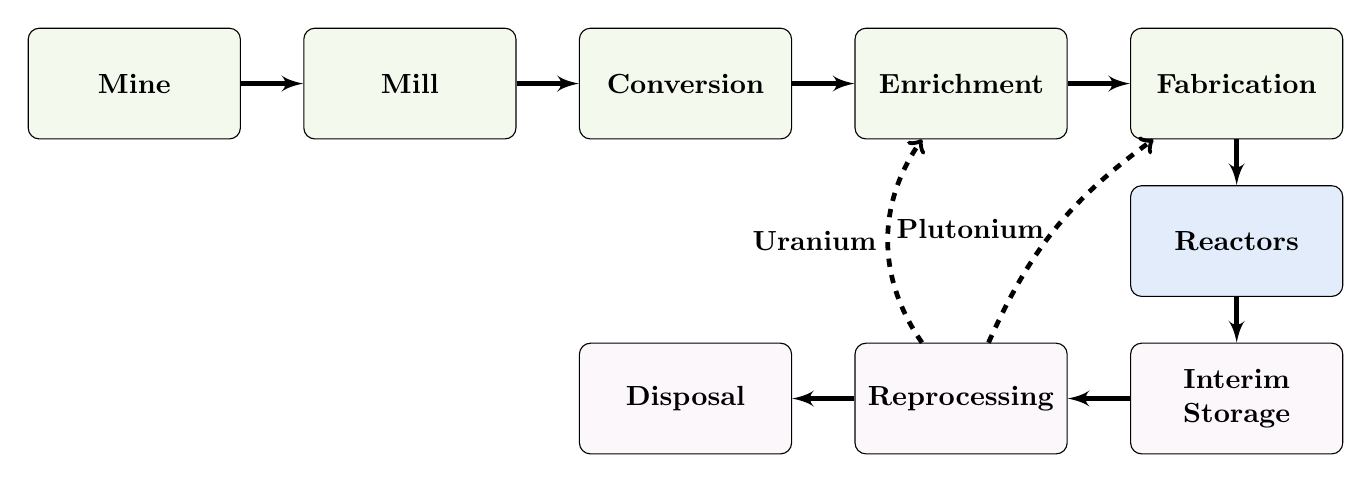
\begin{tikzpicture}
            \node[blockfront] (mine) {\textbf{Mine}};
            \node[blockfront, right of=mine, node distance=3.5cm] (mill) {\textbf{Mill}};
            \node[blockfront, right of=mill, node distance=3.5cm] (conversion) {\textbf{Conversion}};
            \node[blockfront, right of=conversion, node distance=3.5cm] (enrichment) {\textbf{Enrichment}};
            \node[blockfront, right of=enrichment, node distance=3.5cm] (fabrication) {\textbf{Fabrication}};
            \node[blockreactor, below of=fabrication, node distance=2cm] (reactor) {\textbf{Reactors}};
            \node[blockback, below of=reactor, node distance=2cm] (interim) {\textbf{Interim Storage}};
            \node[blockback, left of=interim, node distance=3.5cm] (reprocessing) {\textbf{Reprocessing}};
            \node[blockback, left of=reprocessing, node distance=3.5cm] (disposal) {\textbf{Disposal}};

            \path [line, line width=0.6mm] (mine) -- (mill);
            \path [line, line width=0.6mm] (mill) -- (conversion);
            \path [line, line width=0.6mm] (conversion) -- (enrichment);
            \path [line, line width=0.6mm] (enrichment) -- (fabrication);
            \path [line, line width=0.6mm] (fabrication) -- (reactor);
            \path [line, line width=0.6mm] (reactor) -- (interim);
            \path [line, line width=0.6mm] (interim) -- (reprocessing);
            \path [line, line width=0.6mm] (reprocessing) -- (disposal);

            \draw[dashed, ->, line width=0.6mm] (reprocessing) edge[bend left=15] node[left]{\textbf{Plutonium}} (fabrication);
            \draw[dashed, ->, line width=0.6mm] (reprocessing) edge[bend left=35] node[left]{\textbf{Uranium}} (enrichment);
      \end{tikzpicture}
      \caption{Hypothetical closed fuel cycle where the front end of the fuel cycle results in an initial fuel form, which moves to the reactor before entering the back end of the fuel cycle for reprocessing and disposal. The top row in green represents the front end of the fuel cycle, the middle row in blue represents the reactor fleet, and the bottom row in purple represents the back end of the fuel cycle.}
      \label{fig:closed_fc}
\end{figure}

% \begin{figure}[H]
%       \centering
%       \includegraphics[scale=0.55]{images/nfc/closed_fc.png}
%       \caption{Hypothetical closed fuel cycle.}
%       \label{fig:closed_fc}
% \end{figure}


\subsection{Front End of the Fuel Cycle}
\label{sec:front_end}
The \gls{nea} and \gls{iaea} publish a biennial report on the state of the global uranium market, called the \textit{Red Book}. At the time of writing the 2024 \textit{Red Book} is not public; however, interested parties can extrapolate trends from the 2022 \textit{Red Book} report on global Uranium availability, which covers January 2019 to January 2021 and updates the projections from 54 countries of their uranium supply and resources through 2040 \cite{nea_red_book_2022}.

Globally, Australia holds the most significant reasonably assured resources
of uranium at roughly 28\% of the world's total. However, total identified recoverable resources declined 2\% from 2019 to 2021--in contrast with slight increases reported in previous versions of the report--as countries increased mining efforts, reclassified economic viability of inferred resources, and currency values fluctuated with inflation. Among the most well-established uranium exporters like Australia, Canada, and Kazakhstan, re-evaluations of inferred resources accounted for decreases in nearly every quality category, while relatively new exporters, Mongolia and Niger, reported increases in inferred resources \cite{nea_red_book_2022}. This thesis focuses on the \gls{usa} explicitly and does not incorporate geospatial information, as such it does not present the real limitations of an international fuel cycle.

The \gls{usa} imports more uranium than it produces domestically, as shown in Figure \ref{fig:foregin_u3o8}, from countries with large uranium deposits like Canada, Australia, and Kazakhstan. This trend is expected to continue as investments from the \gls{usa} in new uranium mines could change the domestic availability of uranium ores.

\begin{figure}[H]
   \centering
   \includegraphics[scale=0.7]{images/intro/uranium_production_imports.pdf}
   \caption{Foreign and domestic uranium purchases over time. Reproduced from \cite{eia_monthly_energy_review_2024}.}
   \label{fig:foregin_u3o8}
\end{figure}

As the 2022 \textit{Red Book} notes, the literature surrounding the understanding of best practices for environmental stewardship and remediation of mines is growing. Once-common practices of strip, pit, and underground
mining are beginning to be replaced with more sustainable practices that
minimize the environmental impact of mining. One method that has garnered
interest in the uranium mining community is in-situ leaching, wherein automatic pumps inject a leaching solution into the ground to dissolve the uranium and then pump the solution to the surface for processing \cite{insitu_review_2024}. In-situ leaching is limited to areas with favorable permeabilities, but the reduced labor intensity, simplified infrastructure requirements, and lower environmental impact make it an attractive option for uranium mining where applicable.

In-situ leaching also reduces the extent of the milling process as the ratio of
desirable material to non-desirable material is higher in the leaching solution
than in the resultant material from traditional mining. The milling process
generally involves crushing the ore into a fine powder and then leaching the
uranium from the ore with a sulfuric acid solution. Workers then extract the
uranium from the solution and convert it into yellowcake ($U_3O_8$), a
concentrated form of uranium oxide \cite{milling_uranium_2022}. The yellowcake
is then shipped to a conversion facility, where it is converted into uranium
hexafluoride ($UF_6$), a gas that cools to a liquid and then a solid before it
is transported to be enriched. Uranium hexafluoride is attractive in the
enrichment process because fluorine has only one naturally occurring isotope
and is easy to ensure isolation from the uranium.

Up to the enrichment stage of the fuel cycle, the process is almost entirely
agnostic to the end use of the uranium fuel. Leaving the conversion stage,
$UF_6$ enters the enrichment process aims to achieve a specific concentration
or weight percent of $^{235}$U relative to the other uranium isotopes. Today,
enrichment relies on centrifuges, which separate the isotopes based on their
mass; however, historical gaseous diffusion technology could potentially use
laser enrichment if it becomes economically viable. This thesis does not
distinguish between enrichment services; instead, using \gls{swu}, which Section
\ref{sec:swu} expands on, to quantify the enrichment delivered.

The enriched $UF_6$ is then converted into uranium dioxide ($UO_2$) and
fabricated into fuel. For the \gls{usa} fleet of large \glspl{lwr}, the fuel is made into pellets, stacked into rods, and collected into assemblies. This is not the case for every reactor design, as some reactors use prismatic, pebble, or liquid fuel elements. As with enrichment, the fabrication stage of the fuel cycle is simplified in this thesis, and this thesis does not incorporate explicit details of the fabrication process.

\subsection{Reactor Operation}
\label{sec:reactor_operation}
Up to now, this section has laid out the front end of the fuel cycle. The part of the \gls{nfc} where the fuel is used in the reactor is neither at the front nor back of the fuel cycle. Inside the reactor core, the fuel generates heat through fission, which produces steam, thereby driving a turbine to generate electricity. The fuel remains in the reactor for several years, depending on the reactor design and fuel enrichment, after which possesses different properties leading to new storage and transportation challenges. % This interstitial phase of the \gls{nfc} is now complete.


\subsection{Back-End of the Fuel Cycle}
\label{sec:back_end}
% used fuel storage
After the fuel has been in the reactor for several years, it is removed and
stored in a spent fuel pool. After cooling, the fuel is moved to dry cask
storage, where it will remain until a long-term solution is implemented.
This thesis does not focus on closed-fuel cycles, therefore it does not consider fuel reprocessing in this description of the \gls{nfc}. Instead, it examines the masses of different used fuels to characterize how the current \gls{usa} \gls{nfc} would perform over time with the deployment of new reactors.

% How is radioactive waste managed and disposed of?
When considering a long-term repository for the used fuel, maintainers must consider the macroscopic and microscopic effects of the environment on the repository. On a macroscopic level, climate change will drive shoreline erosion, permafrost recession, and congenital ice sheet melting. Translating these well-known effects into chemical consequences that dictate the design of a repository will require site-specific adaptations on several fronts. Special attention must be given to the impact in the first few thousand years, as this period will exhibit the highest activity. In the case of meltwater exposure, water saturated with dissolved $O_2$ could infiltrate a repository, potentially altering the oxidizing conditions \cite{gurban_hydrochemical_2001}. Consequently, regulators considering the 100,000-year perspective of a potential repository must account for proximity to such meltwater sources to meet the demands imposed by a changing climate.

Sites experiencing reducing conditions may continue to do so; however, the changing climate will also influence the salinity of groundwater. Changes in salinity affect density, which could either exacerbate or mitigate the spread of contaminants in the event of exposure outside the repository \cite{gurban_hydrochemical_2001}. This change in salinity also has the potential to interact differently with canisters, necessitating that proactive regulators ensure containment is designed to withstand a changing environment over the repository's lifetime.

An additional layer of microscopic consideration for these regulatory concerns
is the imminent deployment of new nuclear fuels with different compositions and
forms. Some fuels are designed with pyrolytic carbon matrices that can
immobilize decay products for much longer than current fuel forms. As new fuel
technologies are deployed, \gls{nfc} facilities will need to adapt their
capacities, production timelines, and regulatory compliance. These changes,
although seemingly slight (the fuel will likely still be uranium-based), can
have significant consequences over 100,000 years of storage
\cite{hyland_post_closure_2013}.

\section{\cyclus}
\label{sec:cyclus}
% fix that, too informal and introduces archetypes without context.
\cyclus is an agent-based \gls{nfc} simulator that is versatile, open source, and modular. The software achieves this versatility through a series of generic archetypes that are primarily transaction based. Over the years, the user community and developers have created a litany of nuclear specific archetypes for everything from proliferation assessment to fuel burnup. Many standard fuel cycle facilities have been implemented in the \cycamore repository on GitHub, which holds technology-agnostic archetypes for material sources, material sinks, enrichment services, separations capabilities, and a generic reactor.

% discuss recipes
As \cyclus is a transactions code and not necessarily a physics code,
the reactors incorporate reactor physics through pre-defined "recipes,"
where the user specifies the isotopic concentration of the fresh and
used fuel.

Users approximate the burnup of each fuel element with the
same input recipe as the same; however, in this work we incorporate a
cascading enrichment from \gls{leu+} to \gls{haleu}.
% find a citation or source that companies are actually going to do that
% (best case scenario is find it for each reactor you do it for)

% discuss EVER and CLOVER?
Novel in this work is our use of a low fidelity archetype based on the
\cycamore reactor %\cite{the summer poster}. \gls{ever}

\gls{ever} allows the user to specify multiple recipes for the fuel and
change between them at specific times.


% discuss DRE
As we have discussed, \cyclus's primary function is to keep track of
material transactions between agents. This is accomplished through the
\gls{dre}, which functions like a market where each agent brings a bid
for what and how much material they need and suppliers are matched with
buyers % cite something here.


\subsection{Archetypes and Time Management}
\label{sec:archetypes_and_time_management}

Throughout the \cyclus ecosystem, archetypes interact with the \gls{dre} and each other in a fixed, user defined, time step, forcing the entire simulation to operate on the smallest universal time step. For example, if a fabrication facility can produce material every 2 months but the enrichment facility can only provide material every 3 months, then we would need to use a 1 month time step to capture both. When the time step is smaller than the minimum for a given facility, that facility still participates in the \gls{dre} with a 0 bid. These zero bids, across hundreds of facilities, add complexity and inefficiencies to solving the transaction problem at each time step.

Examining the \cyclus ecosystem, we identified an archetype called $Pattern_Sink$ wherein the user can alter the frequency that the material sink, often called the repository, can accept material. We have created an example of this archetype in action with a simple A-B-C scenario, shown in Figure \ref{fig:a-b-c}. In this scenario, material is received from a source (A) to a reactor (B) with a final (C) sink that can only accept material at a certain frequency.

\begin{figure}
    \centering
    \includegraphics[scale=0.4]{images/cyclus/a-b-c.png}
    \caption{Simple A-B-C Scenario}
    \label{fig:a-b-c}
\end{figure}

If we track the material being received by the sink it becomes clear that this frequency simply alters how frequently the archetype updates its internal understanding of time. As a consequence, it appears in Figure \ref{fig:pattern_freq_50} as though multiple groups of material are received in one time step despite this archetype not having an idea of individual shipments. The way this archetype accomplishes the artificial restriction on accepting material is by simply not updating the time step that the archetype is at until the next universal time step is met. Regardless of function, this is the only example of flexibility of timestep we found in the ecosystem.

\begin{figure}
    \centering
    \includegraphics[scale=0.4]{images/cyclus/pattern_sink_fuel_transactions.pdf}
    \caption{Production of $^{239}$Pu with a frequency of 50 months}
    \label{fig:pattern_freq_50}
\end{figure}

In this work we implement a fundamental toolkit capability that any archetype in the Cyclus ecosystem can take advantage of with one implementation.


\section{LEU Plus}
\label{sec:leup}

As there are various definitions for each class of enrichment, we will use the following for the purposes of this work:

\begin{table}[H]
   \centering
   \caption{Enrichment levels and their ranges.}
   \label{tab:enrichment_levels}
   \begin{tabular}{c c}
      \hline
      \textbf{Enrichment Level} & \textbf{Range [\%  $^{235}$U]} \\
      \hline
      Natural & < 0.711 \\
      \gls{leu} & 0.711-5 \\
      \gls{leup} & 5-10 \\
      \gls{haleu} & 10-20 \\
      \gls{heu} & $\geq$ 20  \\
      \hline
   \end{tabular}
\end{table}

For a fuel cycle containing \gls{leup}, one of the primary advantages is that it would fall under the same licensing category as \gls{leu} fuel. The \gls{nrc} defines a special nuclear material of low strategic significance \cite{nrc_catiii} as meeting one of three criteria, the most notable of which for our purposes is "(3) 10,000 grams or more of uranium-235 (contained in uranium enriched above natural but less than 10 percent in the U–235 isotope)," \cite{nrc_catiii}. This facility definition is where the upper limit of the \gls{leup} range arises.

To enrich to \gls{haleu}, facilities such as TRISO-X LLC and Kairos Power Atlas Fuel Fabrication Facility must move up a category to special nuclear material of moderate strategic significance (Category II). Thus, \gls{leup} is an attractive intermediary step for servicers wishing to minimize the size of a Category II facility (keeping down costs) as it is the same category we have historically licensed for \gls{leu} fuel enrichment.

Traditional \glspl{lwr} could receive benefits from using \gls{leup} fuel; as outlined by L\'{o}pez-Luna et al. \cite{24_month_cycle_bwr}, incorporating such fuel rods would allow for a 24-month cycle the in the \gls{bwr} design they studied and would reduce the levelized cost of the nuclear fuel cycle they simulated. In October 2024, Framatome announced that their 6 wt$\%$ GAIA fuel assemblies completed their third 18-month fuel cycle at the Vogtle plant in Georgia \cite{framatome_press_2024}, with the eventual goal of this process being commercialization of new accident tolerant fuels that can potentially support \gls{leup}. The small, but growing, body of work indicates that \gls{leup} fuels are gaining traction in a variety of technologies; however, the fuel does not exist in a vacuum.

Increased prevalence of higher enrichment fuels will require modifications to the existing supply chain, particularly to ensure continued safety of workers and the public. A 2022 report from Shaw and Clarity out of \gls{ornl} highlighted that existing nuclear fuel vault configurations at \glspl{bwr} and \glspl{pwr} did not have sufficient margins to satisfy regulatory requirements when fully flooded \cite{leup_atf_storage_impacts}. Their report only studied the impacts of 6.5 wt$\%$ and 8 wt$\%$, which they highlight strain existing regulatory limits, and they conclude their report noting that \gls{haleu} fuel would require significant changes to existing fuel storage infrastructure.

\section{TRISO Fuel}
\label{sec:triso_fuel}

In this work, we adapt the approach of Bachmann et \textit{al.} \cite{bachmann_enrichment_2021} to focus on \gls{triso} fueled reactor designs alongside traditional fuel forms at various enrichments. \gls{triso} is not a classification of enrichment, and as such, there are several reactors that make use of different fuel enrichment. As there are various definitions for each class of enrichment, we will use the following for the purposes of this work:

\begin{table}[htbp]
   \centering
   \caption{Enrichment levels and their ranges.}
   \label{tab:enrichment_levels}
   \begin{tabular}{c c}
      \hline
      \textbf{Enrichment Level} & \textbf{Range [\%  $^{235}$U]} \\
      \hline
      natural uranium & < 0.711 \\
      \gls{leu} & 0.711-5 \\
      \gls{leu+} & 5-10 \\
      \gls{haleu} & 10-20 \\
      \gls{heu} & $\geq$ 20  \\
      \hline
   \end{tabular}
\end{table}

The \gls{triso} fuel fabrication process is a complex process that involves multiple steps. We have outlined the general process of producing the fuel in Section \ref{sec:nfc}, here we will distinguish \gls{triso} from the traditional metalic fuels used in \glspl{lwr}.


The process begins with the production of \gls{triso} particles, which are then coated with multiple layers of pyrolytic carbon and silicon carbide. The coated particles are then loaded into fuel compacts, which are then loaded into fuel elements. The fuel elements are then loaded into fuel assemblies, which are then loaded into the reactor core.

\section{Reactor Models}
\label{sec:reactor_models}

This thesis explores various transition scenarios for the deployment in the \gls{usa} of the: 1) \gls{xe} \gls{htgr}; 2) \gls{usnc} \gls{mmr} \gls{htgr}; and 3) and Westinghouse AP1000 \gls{pwr}. To accommodate the assumption that the \gls{haleu}-fueled \gls{triso} reactors will first accept \gls{leup} fuel, this thesis adapts Bachmann's \gls{mmr}-like Serpent model \cite{bachmann_mmr_like_2023} and Richter's \gls{xe}-like Serpent model \cite{richter_xe100_like} to accept \gls{leup} fuel. These reactor models are constructed from publicly available data to approximate their aggregate behavior.

Table \ref{tab:ar_defs} shows the design specifications for the advanced reactors in this thesis. The \gls{mmr} and \gls{xe} reactors are \gls{htgr}s that use \gls{triso} fuel, while the AP1000 is a \gls{pwr} that uses UO$_2$ fuel. The enrichment distinguishes the versions of the \gls{mmr} and \gls{xe} as the only distinguishing variable between the two versions of the reactors. The cycle length, discharge burnup, and reactor lifetime are the same for both versions of the reactors. The AP1000 is assumed to use \gls{leu} fuel throughout the simulation. The \gls{mmr} is the smallest power output reactor in this thesis, and can serve as a representative of mix of small, \gls{triso}-fueled reactors. The \gls{xe} reactor is an order of magnitude larger in power output, and can be considered a representative of larger, \gls{triso}-fueled reactors. The AP1000 is the largest reactor in this thesis and is a representative of gigawatt-scale reactors.


\begin{table}[H]
   \centering
   \caption{Advanced reactor design specifications.}
   \label{tab:ar_defs}
   \begin{tabular}{l l l l}
      \hline
      \textbf{Design Criterion} & \textbf{MMR-Like} \cite{usnc_design_2021} & \textbf{\gls{xe}-Like} \cite{nuscale_chapter_2018} & \textbf{AP1000} \\
      \hline
      Reactor type & \gls{htgr} & \gls{htgr} & \gls{pwr} \\
      Power Output [MWe] & 15 & 100 & 1000 \\
      Fuel Type & \gls{triso} & \gls{triso} & UO$_2$ \\
      Enrichment [\% $^{235}$U] & 9.95, 19.75 & 9.95, 15.5 & 5 \\
      Cycle Length & 20 [yrs] & Online Refuel & 18 [months] \\
      Discharge Burnup [GWd/MTU] & 82 & 168 & 65 \\
      Reactor Lifetime [yrs] & 20 & 60 & 60 \\
      \hline
   \end{tabular}
\end{table}

The following subsections discuss the reactors in greater detail. These models  approximate that the \gls{leup}-fueled reactors achieve the same burnup, power level, and core lifetime as the \gls{haleu}-fueled version. These assumptions are sufficient for the metrics outlined in Section \ref{sec:metrics} as this thesis does not perform \gls{uf} isotopic analysis, but could stretch the \gls{uf} temporal profile.



\subsection{MMR-like Reactor}
\label{sec:mmr}

In 2021, \gls{uiuc} submitted a notice of intent to the \gls{nrc} detailing their plans to apply for a construction permit of the \gls{mmr} reactor from \gls{usnc} \cite{uiuc_notice_nrc_2021}. Activities have continued as \gls{uiuc} continues the project, they reached the pre-licensing phase with the \gls{nrc} and were planning on commencing operation of an on-campus reactor in the 2030s. This \gls{mmr} is an \gls{htgr} that uses \gls{triso} fuel, has an electrical output of 15 MW$_e$, and a cycle length of 20 years. The fuel is enriched to 9.95\% $^{235}$U for \gls{leup} and 19.75\% for \gls{haleu}. As modeled, both have a discharge burnup of 82 GWd/MTU, which coincides with the 20-year lifetime of the reactor. In this thesis, the \gls{mmr} is based on the model developed by Bachmann et al. \cite{bachmann_mmr_like_2023} and is implemented here as-is for the \gls{haleu} version of the reactor, while the \gls{leup} version updates the fuel composition from the \gls{haleu} version.

Figure \ref{fig:mmr_design} shows a rendering of the \gls{mmr} core and reactor vessel. As indicated by the figure, the design is intended to be underground, with an estimated total reactor footprint less than 5 acres. The primary coolant is helium gas, which heats up in the core and deposits its heat in a heat exchanger to generate electricity to the side of the reactor \cite{usnc_chalk_river}. Helium is transparent to many nuclear interactions and is inert, making it an attractive choice for a coolant.

\begin{figure}[H]
    \centering
    \includegraphics[scale=0.19]{images/reactor_design/wide-02.png}
    \caption{USNC MMR design \cite{usnc_design_2021}.}
    \label{fig:mmr_design}
\end{figure}

The proposed deployment of this reactor concept includes an operational \textit{\gls{mmr} Energy System} consisting of two plants: the \textit{Nuclear Plant} and the \textit{Adjacent Plant}. The \textit{Nuclear Plant} contains multiple \gls{mmr} units, including all the equipment required to transport the heat to the \textit{Adjacent Plant}. The \textit{Adjacent Plant} consists of the equipment that converts heat to electricity or process heat as needed. The \textit{\gls{mmr} Energy System} will theoretically store up to 10 hours of power plant thermal output and can be supplemented with hydrogen burners. Auxiliary molten salt thermal storage allows for a flexible electricity and process heat supply.

Electricity and heat would be delivered on demand from the power plant while the \gls{mmr} unit operates at constant power. The \gls{mmr}'s high-temperature heat has many uses beyond the generation of electricity. District heating, desalination, and chemical or industrial heat highlight the broader point of how \gls{geniv} nuclear reactors are not solely intended for electricity generation as with the current domestic fleet. An \gls{mmr} could deliver steam temperatures of 660 °C, and they estimate that temperatures up to 950 °C could be possible in future \gls{mmr} variants \cite{usnc_design_2021}.

The fuel for this reactor is inspired by the \gls{triso} fuel developed in the 1960s and 1970s. A small sphere of uranium fuel is coated in carbon and silicon carbide layers. As shown in Figure \ref{fig:usnc_fuel}, the fuel is composed of kernels arranged into a larger fuel pellet. They call their fuel form \gls{fcm} fuel. They additively manufacture each element, allowing for a high packing fraction of fuel, which means their fuel could be adapted to other reactor designs.

\begin{figure}[H]
    \subfloat[Fuel element layers.\label{fig:elemenet_layers}]{%
      \includegraphics[width=0.49\textwidth]{images/reactor_design/usnc_triso.png}
   }
    \hfill
    \subfloat[Fuel pellet profile.\label{fig:pellet_profile}]{%
      \includegraphics[width=0.49\textwidth]{images/reactor_design/usnc_fuel_side.jpeg}
   }
    \caption{
    USNC \gls{mmr} fuel renderings
      \cite{usnc_media_kit}.}
    \label{fig:usnc_fuel}
\end{figure}

Figure \ref{fig:mmr_core} shows a top-down and side view of the \gls{mmr} Serpent model \cite{bachmann_mmr_like_2023}, modified in fuel composition alone. As Bachmann describes \cite{bachmann_thesis_2023}, the radius of the fuel channel is based on the publicly available size of the \gls{fcm} pellets (1.15 cm), and the coolant channel has an arbitrarily chosen radius of 3 cm. The entire core is assumed to be in an isothermal state at 800 K. There is a 20 cm thick graphite reflector above and below the stacks of graphite and a 10 cm thick beryllium-oxide reflector on the outside of the graphite blocks of the core, illustrated by the green material in Figure \ref{fig:mmr_core}. The model does not contain control rods or burnable poisons, so the control rod tubes are filled with helium. Five layers of graphite fuel blocks are stacked to form the entire core to approximate the number of fuel blocks described in the publicly available data \cite{usnc_design_2021}. The fuel does not move through the core, as the model is designed to use the same fuel for the entire reactor lifetime.


\begin{figure}[H]
    \subfloat[Top-down core view.\label{fig:mmr_td}]{%
      \includegraphics[width=0.49\textwidth]{images/reactor_design/haleu_mmr_2blocks.inp_geom1.png}
   }
    \hfill
    \subfloat[Full core side profile.\label{fig:mmr_slice}]{%
      \includegraphics[width=0.49\textwidth]{images/reactor_design/haleu_mmr_2blocks.inp_geom3.png}
   }
    \caption{Serpent model of the USNC MMR core.}
    \label{fig:mmr_core}
\end{figure}



\subsection{Xe-100-like Reactor}
\label{sec:xe}

X-Energy has entered into a cooperative agreement with \gls{doe} to deploy their \gls{xe}, is in the pre-licensing phase with the \gls{nrc} for projects in Texas and Washington, and is expected to be operational in the 2030s. There are similar projects in the early stages in Canada and the \gls{uk}. The X-Energy \gls{xe} is an \gls{htgr} that uses \gls{triso} fuel and is expected to operate for 60 years. The reactor has an electical output of 100 MW and uses online refueling. The fuel is enriched to 9.95\% $^{235}$U for \gls{leup} and 15.5\% $^{235}$U for \gls{haleu} and a discharge burnup of 168 GWd/MTU. The reactor in this thesis is an approximation based on publicly available data and is not based on confidential or proprietary information. The model was developed by Richter et al. \cite{richter_xe100_like} and is implemented herein as-is for the \gls{haleu}-fueled reactor, while the \gls{leup} version has a modified fuel composition.

Figure \ref{fig:xe_design} shows a rendering of the \gls{xe} core and reactor vessel. The \gls{xe} reactor is designed to be a small modular reactor that can be deployed in various locations and will be gas-cooled. This design differs from the \gls{mmr} as the reactor features online refueling.

\begin{figure}[H]
    \centering
    \includegraphics[scale=0.09]{images/reactor_design/xe-100-reactor-slice.jpg}
    \caption{X-Energy Xe-100 rendition \cite{xe_reactor}.}
    \label{fig:xe_design}
\end{figure}

Unlike the \gls{mmr}'s annular fuel elements, the \gls{xe} pebbles are composed of a spherical graphite matrix that contains the \gls{triso} fuel particles. These \gls{triso} particles are similar to those in the \gls{mmr}, as shown in Figure \ref{fig:xe_fuel}.

\begin{figure}[H]
    \centering
    \includegraphics[scale=0.28]{images/reactor_design/graphic-triso-x-pebble.jpg}
    \caption{X-Energy Xe-100 fuel pebble \cite{xe_fuel}.}
    \label{fig:xe_fuel}
\end{figure}


This thesis modifies the fuel composition of Richter's \gls{xe}-like reactor model to accept \gls{leup} fuel. The \gls{leup} fuel is assumed to have the same burnup and power level as the \gls{haleu} fuel. This assumption, as with the \gls{mmr}-like reactor, would impact the \gls{uf} isotopic calculations. I will explore the implications in future work. Figure \ref{fig:xe_core} shows the top-down view of the \gls{leup} \gls{xe} core as the \gls{haleu} version has been established by Richter \cite{richter_thesis_2022}.

\begin{figure}[H]
    \subfloat[Initial core. \label{fig:xe_init_core}]{%
      \includegraphics[width=0.49\textwidth]{images/reactor_design/htgr-mr-burn-200.inp_mesh1_bstep0.png}
   }
    \hfill
    \subfloat[Final core. \label{fig:xe_final_core}]{%
      \includegraphics[width=0.49\textwidth]{images/reactor_design/htgr-mr-burn-200.inp_mesh1_bstep6.png}
   }
    \caption{Top-down view of the \gls{leup} X-Energy Xe-100 core model where darker shading corresponds to higher burnup, and lighter shading corresponds to lower burnup.}
    \label{fig:xe_core}
  \end{figure}

Figures \ref{fig:xe_init_core} and \ref{fig:xe_final_core} are shaded based on the burnup of the fuel, with darker pebbles indicating higher burnup. The pebbles are inserted into the core at the top, and gravity pulls them down through the core. After a brief holding time outside the core, the pebbles are reinserted at the top of the core. In \cyclus, we approximate the core as containing 6 batches in the core and one batch is removed when they reach the end of their life. This process is repeated until the pebbles reach their targeted number of passes, at which point they are removed from the core and stored.

\subsection{AP1000 Reactor}
\label{sec:ap}

AP1000s are operational in the \gls{usa} and China, and the \gls{uk} and India plan to deploy more. The Westinghouse AP1000 is a \gls{pwr} that uses UO$_2$ fuel. The reactor has an electrical output of 1000 MW, a cycle length such that every 18 months 80 fuel assemblies are replaced, and an expected lifetime of 60 years. The fuel is enriched to approximately 5\% $^{235}$U and has a discharge burnup of 65 GWd/MTU. The reactor in this thesis is an approximation based on publicly available data about the units currently operating at the Vogtle Plant in Georgia, and is not based on confidential or proprietary information. As this thesis does not anticipate \gls{leup} being used in the AP1000, there is no such neutronics model of the reactor herein, and this work adapts the generic \cycamore reactor archetype to represent the AP1000 in number of fuel assemblies, power output, core mass, and cycle length.



\chapter{Deployment Scenarios}
\label{ch:scenarios}
\glsresetall

In this work we explore the deployment of advanced reactors in the future energy landscape of the \gls{usa}. As the landscape evolves, compounding factors will drive actual deployment of these reactors in ways this work does not capture. The value of energy system modeling, and this type of transition scenario, is to understand the implications of deployment compared with and measured relatively to business as usual cases with similar approximations.

We use this chapter to explore the deployment schemes we have implemented---outlined in Table \ref{tab:deployment_schemes}---, and the demand growth scenarios we have considered---outlined in Table \ref{tab:demand_scenarios}. We will also discuss two additional deployment schemes that were implemented, but not incorporated as they are more useful for problems not considered herein.

\begin{table}[htbp]
    \centering
    \caption{Deployment Schemes}
    \label{tab:deployment_schemes}
    \begin{tabular}{p{0.15\linewidth} p{0.27\linewidth} p{0.50\linewidth}}
        \hline
        \textbf{Status} & \textbf{Scheme} & \textbf{Description} \\
        \hline
        \multirow{3}{*}{Incorporated} & Greedy Deployment & Deploy the largest reactor first at each time step, fill in the remaining capacity with the next smallest, and so on. \\
        & Random Deployment & Uses a date and hour as seed to randomly sample the reactors list. \\
        & Initially Random, Greedy Deployment & Randomly deploys reactors until a reactor bigger than the remaining capacity is proposed for each year, then fills remaining capacity with a greedy algorithm. \\
        \hline
        \multirow{2}{*}{Not Incorporated} & Capped Deployment & There is a single-number capacity for one or more of the reactor models. \\
        & Pre-Determined Distribution Deployment & One or more reactors have a preset distribution, and a smaller capacity model fills in the gaps. \\
        \hline
    \end{tabular}
\end{table}

We apply each of these deployment schemes to a series of demand growth scenarios based on two predictions. The \gls{eia} publishes demand expansion projections for the totality of \gls{usa} .
% source name and citation with

\begin{table}[htbp]
    \centering
    \caption{Demand Growth Scenarios}
    \label{tab:demand_scenarios}
    \begin{tabular}{c c c}
        \hline
        \textbf{Demand Growth} & \textbf{Range} & \textbf{Source}\\
        \hline
        No growth & 0\% & na\\
        Low growth & 1\%, 5\%, 10\%, 15\% & (eia)\\
        High growth & 100\%, 200\% & (liftoff)\\
        \hline
    \end{tabular}
\end{table}

\section{Greedy Deployment}
% describe the algorithm in detail
In this deployment scheme, the largest reactor is deployed first until another
deployment of that reactor would exceed the demand. Then the next largest
reactor is deployed in the same pattern until the next deployment of the
smallest reactor would exceed the demand. This scheme is not a proxy for
strategic decisions by individual actors, it merely meets the demand in a
roughly efficient manner.

\begin{figure}[!htbp]
    \centering
    \includegraphics[scale=0.4]{images/schemes/greedy_diagram.png}
    \caption{Greedy Deployment Diagram}
    \label{fig:greedy_diagram}
\end{figure}

% what are the realistic and the unrealistic parts

% when does it over or under perform


\section{Random Deployment}
% describe the algorithm in detail

% what are the realistic and the unrealistic parts
Advanced reactor concepts, like the ones outlined in this work, are often designed for a different use-cases. ((((((((((((cite))))))))))))


The deployment of these reactors is a complex problem that requires a nuanced
understanding of the energy market, the regulatory environment, the intended
use of the technology, and the technical capabilities of the reactor. This
random deployment is a proxy for the complexity of the real-world deployment
problem, but does not include the nuance of future user needs, which will drive
the strategic decisions that utilities and rate payers behind the meter make in
their reactor choices.

This deployment scheme has the potential to capture some of the complexities in
overall market development, but the extent that these details are captured is
not explored in this work. %%% Should I? I'm not sure how long this would take to do, maybe something with ORSAGE?

\begin{figure}[!htbp]
    \centering
    \includegraphics[scale=0.4]{images/schemes/random_diagram.png}
    \caption{Random Deployment Diagram}
    \label{fig:random_diagram}
\end{figure}

% when does it over or under perform


\section{Initially Random, Greedy Deployment}
% describe the algorithm in detail

\begin{figure}[!htbp]
    \centering
    \includegraphics[scale=0.4]{images/schemes/random_diagram.png}
    \caption{Initially Random, Greedy Deployment Diagram}
    \label{fig:init_random_greedy_diagram}
\end{figure}

% what are the realistic and the unrealistic parts

% when does it over or under perform


\section{Considered Deployment Schemes}

In addition to the deployment schemes outlined above, we also considered a few other deployment schemes that were not included in the final analysis. These schemes were considered for their potential to capture the complexity of the deployment problem, but were ultimately not included due to the egregious nature of approximation required to make the implementation or the lack of a clear benefit over the other schemes.

\subsection{Capped Deployment}
% describe the algorithm in detail
In this scheme, there is a constant limit placed on the number of a specific reactor that can be deployed at any given time step. This is a simple way to model aggregate supply chain constrains that could limit vendors from deploying reactors freely. With the right constraints, this scheme would better succeed at roughly incorporating the limits of a workforce over a short to medium time scale. As workforce constraints are outside the scope of this work, this scheme was implemented but not incorporated in this work.

To use this deployment scheme, a user needs some idea of the supply chain constraints that will limit the deployment of the reactors they are deploying. In Figure \ref{fig:cap_diagram}, we illustrate the defining steps of the capped deployment scheme. The main loop in the logic is consistent with the greedy deployment scheme, but adds a check to see if the current deployment exceeds the limit on that model. If it does, the reactor is removed from the list of reactors to be deployed in that time step.

\begin{figure}[!htbp]
    \centering
    \includegraphics[scale=0.4]{images/schemes/cap_diagram.png}
    \caption{Capped Deployment Diagram}
    \label{fig:cap_diagram}
\end{figure}

% what are the realistic and the unrealistic parts
The realism of this deployment scheme mirrors some elements of the pre-determined distribution (this is a flat distribution after all), but the cap is a less granular way to account for supply chain constraints

% when does it over or under perform

\section{Pre-Determined Distribution Deployment}
% describe the algorithm in detail
This deployment scheme allows users to incorporate the projections and
commitments of rate payers and utilities by setting a distribution over the
time of the simulation. In this scheme the distribution serves as a cap to the
number of reactors deployed in a time step, and reactors are preferentially
deployed first to meet those caps. After that has been completed, the remaining
reactors without caps are deployed to meet the demand. In this way, we are able
to incorporate knowledge of supply chain constraints for specific technologies
without having to model the supply chain in detail.
% would be great to find some sources for this, and see what the literature says

\begin{figure}[!htbp]
    \centering
    \includegraphics[scale=0.4]{images/schemes/pre_det_diagram.png}
    \caption{Pre-Determined Distribution Deployment Diagram}
    \label{fig:pre_det_diagram}
\end{figure}

% what are the realistic and the unrealistic parts

% when does it over or under perform
This scheme is most useful when there are known commitments to specific technologies.

\section{Metrics}
\label{sec:metrics}

% discuss the metrics you are using
In this work, we will develop a model of nuclear energy in the \gls{usa} using concepts from \glspl{esm} on scenarios that compare the transition from our current fleet to incorporate advanced reactor technologies not currently deployed. To compare these scenarios, we have chosen to focus on a few key metrics: \gls{swu}, energy output, mass of fuel, and reactor deployment.

\subsection{Separative Work Units}
\label{sec:swu}

\gls{swu}, or Separative Work Units, is a ubiquitous measure of effort
that goes into producing nuclear fuel. It is simplified as:
\begin{align}
    SWU&= Q(C_p-C_f)
    \intertext{Where:}
    SWU&= \mbox{Separative Work Units [kgSWU]}\nonumber\\
    Q&= \mbox{ Quantity of material processed [kg]}\nonumber\\
    C_p&=\mbox{ Enrichment level of the product [$\%$]}\nonumber\\
    C_f&= \mbox{ Enrichment level of the feed [$\%$].}\nonumber
\end{align}

In this work, we will compare the \gls{swu} required for each scenario to understand the relative effort required to deploy the reactors and provide a stable precursor to economic calculations.

\subsection{Energy Output}
\label{sec:energy_output}

% just spit balling
The deployment of reactors in this work is based on energy demand, which
approximates the complicated relationship that generators and utilities
have with power expansions.

The reactors simulated herein have a static peak energy output, so the
nuance in the fleet's ability to meet the demand comes from the
deployment scheme and limitations in the fuel supply chain.

We have created a toy scenario to understand the ways in which the
deployment schemes under and over perform, and we will devote time to
discussing the realistic features of each scheme.

% sensitivity analysis?

\subsection{Mass of Fuel}
\label{sec:mass_of_fuel}

\cyclus has an understanding of the mass of material in each
transaction, in this work we will couple this tracking with an idea of
the volume of the fuel elements to get a relative sense of the volume
each scenario would produce.

We will further compare this with the storage capacity of proposed
projects in the \gls{usa}--like Yucca Mountain.
% improve with comprehensive list

In addition to the volume, the mass % sensitivity analysis?

\section{Greedy Deployment}
\label{sec:greedy_deployment}

In this scheme, we deploy the largest reactor first until another
deployment of that reactor exceeds the demand---as outlined in
\ref{fig:greedy_diagram}. Then we move to the next largest reactor until the
next deployment of the smallest capacity reactor exceeds the
demand. This scheme is not a proxy for strategic decisions by individual
actors it merely meets the demand in a roughly efficient manner.

Previous work from Bachmann et al. \cite{bachmann_enrichment_2021}
employed a similar scheme to explore the deployment of advanced
reactors in the \gls{usa}. This scheme is computationally efficient and allows
for the exploration of the deployment of advanced reactors in a way that is not
overly complex. This scheme is most useful for scenarios where the user is
interested in comparing metrics relative to the number of specific reactors
deployed outside of the context of the problem.

\begin{figure}[H]
    \centering
    \includegraphics[scale=0.4]{images/schemes/greedy_diagram.png}
    \caption{Greedy Deployment Diagram}
    \label{fig:greedy_diagram}
\end{figure}

Through the greedy deployment, we are not attempting to capture the complexity
of the deployment problem but rather to explore the implications of deploying a
certain number of reactors. As such, we limit the discussion of realism to the
extent that the scheme meets the demand and could mirror large actors in a
market. The scheme will deploy reactors until the demand is met within the
amount of the smallest capacity reactor. In these results, we will show the results for the no growth scenario and the double nuclear by 2050 scenario.

\subsection{Number of Reactors}
\label{sec:greedy_reactors}

As we have noted, one of the most notable differences between the no growth scenario and the doubling scenario is that the transition for the no growth scenario will begin closer to 2050 instead of 2030. This trend is reflected in Figures \ref{fig:greedy_mf_reactors} and \ref{fig:greedy_of_reactors}, where the \glspl{mmr}, \glspl{xe}, and AP1000s start as the existing \gls{lwr} fleet are retired. Comparing across fuel regimes, we see that Figures \ref{fig:greedy_mf_ng_reactors} and \ref{fig:greedy_of_ng_reactors} are identical, which typifies the impact of the delayed transition in the no growth scenario.

% Show total number of reactors multi fuel

\begin{figure}[H]
    \subfloat[No Growth \label{fig:greedy_mf_ng_reactors}]{%
      \includegraphics[width=0.495\textwidth]{images/results/reactors/multi_dgng_reactors.pdf}
   }
    \hfill
    \subfloat[Double \label{fig:greedy_mf_d2_reactors}]{%
      \includegraphics[width=0.495\textwidth]{images/results/reactors/multi_dg2_reactors.pdf}
   }
    \caption{Greedy multi fuel reactor deployment.}
    \label{fig:greedy_mf_reactors}
\end{figure}

% talk about the rate of deployment
A direct consequence of the greedy deployment scheme is that, in the doubling scenario, the AP1000 is deployed the most over time, where as the no growth scenario shows the opposite. Another consequence of the deployment scheme is that the rate of deployment for the single fuel regime compared with the multi fuel regime is identical, and future work could investigate further implications of transitioning from one fuel type to another in regard to operation. Simply meeting energy demand is not how utilities make decisions, and is not the intended use case of the broad generation of new nuclear reactors, so we are able to identify an upper bounding case for the energy demand met by designs like the \gls{mmr} or \gls{xe}.


\begin{figure}[H]
  \subfloat[No Growth \label{fig:greedy_of_ng_reactors}]{%
    \includegraphics[width=0.495\textwidth]{images/results/reactors/one_dgng_reactors.pdf}
 }
  \hfill
  \subfloat[Double \label{fig:greedy_of_d2_reactors}]{%
    \includegraphics[width=0.495\textwidth]{images/results/reactors/one_dg2_reactors.pdf}
 }
  \caption{Greedy single fuel reactor deployment.}
  \label{fig:greedy_of_reactors}
\end{figure}

In Table \ref{tab:greedy_reac_avg} we can see how the average number of reactors by design is not influenced by the interstitial as we have modeled it in this work. Compared to the no growth scenario, the double by 2050 scenario shows a significant increase in the average number of each design operating across the 2030-2104 timeline. Consequently, the average number of the AP1000s increases by 757\% between the two growth scenarios, which is the largest increase of any design. The \gls{xe} reactors show the second largest increase at 163\%, followed by the \gls{mmr} at 109\%.

\begin{table}[H]
  \centering
  \caption{Average greedy total operating reactors by design.}
  \label{tab:greedy_reac_avg}
  \begin{tabular}{c c c c c}
     \hline
     Scenario & No Growth, Single & No Growth, Multi & Double, Single & Double, Multi  \\
     \hline
     \gls{haleu} fueled MMRs      & 131.613 & 131.613 & 274.493 & 257.427 \\
     \gls{leup} fueled MMRs       & --      & --      & --      & 17.067 \\
     \gls{haleu} fueled \gls{xe}s & 94.04   & 94.04   & 246.88  & 184.48 \\
     \gls{leup} fueled \gls{xe}s  & --      & --      & --      & 62.4 \\
     \gls{leu} fueled AP1000      & 38.667  & 38.667  & 331.387 & 331.387 \\
     \hline
  \end{tabular}
\end{table}




\subsection{SWU Results}
\label{sec:greedy_swu}

% talk about the types of category facility
In Figure \ref{fig:swu_yearly_greedy} we can see the yearly \gls{swu} demand periodically spike as the demand for enrichment services grows to meet the fuel demand for the fleet. When reactors begin operation in the depicted no growth scenario around 2050, the \gls{swu} demand for the AP1000 peaks above the other two reactors while the demand from \glspl{xe} exceeds the demand from \glspl{mmr}. This trend is exacerbated in the double by 2050 scenarios shown in Figures \ref{fig:greedy_mf_d2_swu} and \ref{fig:greedy_of_d2_swu} where the \gls{swu} for AP1000 \gls{leu} fuel rises quickly and eventually exceeds the total \gls{swu} for the existing fleet.

% talk about the SWU capacity

% show the total SWU capacity

\begin{figure}[H]
    \centering
    \includegraphics[scale=0.7]{images/results/swu/multi_dgng_swu_by_fuel.pdf}
    \caption{Greedy yearly SWU capacity multi fuel, no growth scenario.}
    \label{fig:swu_yearly_greedy}
\end{figure}

As the features of the yearly data are regular and dictated by the cycles of the reactors, we will visualize the total \gls{swu} demand in the cumulative plots in Figures \ref{fig:greedy_mf_swu} and \ref{fig:greedy_of_swu}.

\begin{figure}[H]
  \subfloat[No Growth \label{fig:greedy_mf_ng_swu}]{%
    \includegraphics[width=0.495\textwidth]{images/results/swu/multi_dgng_swu_cumulative_by_fuel.pdf}
 }
  \hfill
  \subfloat[Double \label{fig:greedy_mf_d2_swu}]{%
    \includegraphics[width=0.495\textwidth]{images/results/swu/multi_dg2_swu_cumulative_by_fuel.pdf}
 }
  \caption{Greedy multi fuel SWU.}
  \label{fig:greedy_mf_swu}
\end{figure}


% talk about international trade

\begin{figure}[H]
  \subfloat[No Growth \label{fig:greedy_of_ng_swu}]{%
    \includegraphics[width=0.495\textwidth]{images/results/swu/one_dgng_swu_cumulative_by_fuel.pdf}
 }
  \hfill
  \subfloat[Double \label{fig:greedy_of_d2_swu}]{%
    \includegraphics[width=0.495\textwidth]{images/results/swu/one_dg2_swu_cumulative_by_fuel.pdf}
 }
  \caption{Greedy single fuel SWU.}
  \label{fig:greedy_of_swu}
\end{figure}

In Table \ref{tab:greedy_swu_avg} we can see the average \gls{swu} demand by design in the no growth and double by 2050 scenarios. The \gls{swu} demand for the \gls{mmr} and \gls{xe} reactors is the same in the single and multi fuel regimes for the no growth scenarios, which is consistent with the reactor deployment trends we have seen in the Section \ref{sec:greedy_reactors}. The \gls{swu} demand for the AP1000s increases by 800\% from the no growth scenario to the double scenario, which is consistent with the reactor deployment trends we have seen in the previous section. The \gls{swu} demand for \gls{xe} \gls{haleu} increases 167\%, while the \gls{swu} demand for \gls{mmr} \gls{haleu} increases 105\% from the no growth scenario to the double scenario.

\begin{table}[H]
  \centering
  \caption{Average greedy yearly SWU by design in k\gls{swu}.}
  \label{tab:greedy_swu_avg}
  \begin{tabular}{c c c c c}
     \hline
     Scenario & No Growth, Single & No Growth, Multi & Double, Single & Double, Multi  \\
     \hline
     \gls{mmr} \gls{haleu}   & 48.699  & 48.699  & 99.974   & 95.127   \\
     \gls{mmr} \gls{leup}    & --      & --      & --       & 2.228    \\
     \gls{xe} \gls{haleu}    & 139.926 & 139.926 & 374.323  & 362.312  \\
     \gls{xe} \gls{leup}     & --      & --      & --       & 7.227    \\
     AP1000 \gls{leu}        & 573.989 & 573.989 & 5167.815 & 5167.815 \\
     \hline
  \end{tabular}
\end{table}



\subsection{Fresh Fuel Results}
\label{sec:greedy_fresh}

% talk about the types of fuel
In Figures \ref{fig:greedy_mf_fresh} and \ref{fig:greedy_of_fresh} we can see the fresh fuel demand for the reactors in the no growth and double by 2050 scenarios. The fresh fuel curves in each scenario follow the same pattern as the reactor deployment curves, as \cyclus supplies fuel to each of the reactors as it is deployed.

% show total fresh fuel

\begin{figure}[H]
  \subfloat[No Growth \label{fig:greedy_mf_ng_fresh}]{%
    \includegraphics[width=0.495\textwidth]{images/results/fresh/multi_dgng_fresh_fuel_cumulative_by_fuel.pdf}
 }
  \hfill
  \subfloat[Double \label{fig:greedy_mf_d2_fresh}]{%
    \includegraphics[width=0.495\textwidth]{images/results/fresh/multi_dg2_fresh_fuel_cumulative_by_fuel.pdf}
 }
  \caption{Greedy multi fresh fuel amount.}
  \label{fig:greedy_mf_fresh}
\end{figure}

% talk about transportation of fuel


\begin{figure}[H]
  \subfloat[No Growth \label{fig:greedy_of_ng_fresh}]{%
    \includegraphics[width=0.495\textwidth]{images/results/fresh/one_dgng_fresh_fuel_cumulative_by_fuel.pdf}
 }
  \hfill
  \subfloat[Double \label{fig:greedy_of_d2_fresh}]{%
    \includegraphics[width=0.495\textwidth]{images/results/fresh/one_dg2_fresh_fuel_cumulative_by_fuel.pdf}
 }
  \caption{Greedy single fresh fuel amount.}
  \label{fig:greedy_of_fresh}
\end{figure}

In Table \ref{tab:greedy_fresh_avg} we can see the average yearly fresh fuel demand by design in the no growth and double by 2050 scenarios. The AP1000 \gls{leu} shows the largest increase in fresh fuel demand from the no growth scenario to the double scenario at 800\%, followed by the \gls{xe} \gls{haleu} at 159\%. The \gls{mmr} \gls{haleu} reactors show the smallest increase in fresh fuel demand at 105\%.


\begin{table}[H]
  \centering
  \caption{Average greedy yearly fresh fuel by design in tonnes.}
  \label{tab:greedy_fresh_avg}
  \begin{tabular}{c c c c c}
     \hline
     Scenario & No Growth, Single & No Growth, Multi & Double, Single & Double, Multi  \\
     \hline
     \gls{mmr} \gls{haleu}   & 1.079    & 1.079   & 2.216    & 2.108    \\
     \gls{mmr} \gls{leup}    & --       & --      & --       & 0.107    \\
     \gls{xe} \gls{haleu}    & 4.059    & 4.059   & 10.859   & 10.511   \\
     \gls{xe} \gls{leup}     & --       & --      & --       & 0.348    \\
     AP1000 \gls{leu}        & 74.636   & 74.636  & 671.976  & 671.976  \\
     \hline
  \end{tabular}
\end{table}



\subsection{Used Fuel Results}
\label{sec:greedy_used}

In Figures \ref{fig:greedy_mf_used} and \ref{fig:greedy_of_used} we can see the used fuel demand for the reactors in the no growth and double by 2050 scenarios. The used fuel curves in each scenario lag the reactor deployment curves, as \cyclus removes the used fuel after the appropriate number of cycles from  each of the operating, and eventually decommissioning, reactors.

% show total used fuel
\begin{figure}[H]
  \subfloat[No Growth \label{fig:greedy_mf_ng_used}]{%
    \includegraphics[width=0.495\textwidth]{images/results/used/multi_dgng_used_fuel_cumulative_by_fuel.pdf}
 }
  \hfill
  \subfloat[Double \label{fig:greedy_mf_d2_used}]{%
    \includegraphics[width=0.495\textwidth]{images/results/used/multi_dg2_used_fuel_cumulative_by_fuel.pdf}
 }
  \caption{Greedy multi used fuel amount.}
  \label{fig:greedy_mf_used}
\end{figure}


\begin{figure}[H]
  \subfloat[No Growth \label{fig:greedy_of_ng_used}]{%
    \includegraphics[width=0.495\textwidth]{images/results/used/one_dgng_used_fuel_cumulative_by_fuel.pdf}
 }
  \hfill
  \subfloat[Double \label{fig:greedy_of_d2_used}]{%
    \includegraphics[width=0.495\textwidth]{images/results/used/one_dg2_used_fuel_cumulative_by_fuel.pdf}
 }
  \caption{Greedy single used fuel amount.}
  \label{fig:greedy_of_used}
\end{figure}

In Table \ref{tab:greedy_used_avg} we can see the average yearly used fuel by design in the no growth and double by 2050 scenarios. The AP1000 \gls{leu} shows the largest increase in used fuel demand from the no growth scenario to the double scenario at 743\%, followed by the \gls{xe} \gls{haleu} at 164\%. The \gls{mmr} \gls{haleu} reactors show the smallest increase in used fuel demand at 154\%.


\begin{table}[H]
  \centering
  \caption{Average greedy yearly used fuel by design in tonnes.}
  \label{tab:greedy_used_avg}
  \begin{tabular}{c c c c c}
     \hline
     Scenario & No Growth, Single & No Growth, Multi & Double, Single & Double, Multi  \\
     \hline
     \gls{mmr} \gls{haleu}   & 0.499    & 0.499   & 1.267    & 1.160    \\
     \gls{mmr} \gls{leup}    & --       & --      & --       & 0.107    \\
     \gls{xe} \gls{haleu}    & 3.714    & 3.715   & 9.826    & 9.477    \\
     \gls{xe} \gls{leup}     & --       & --      & --       & 0.348    \\
     AP1000 \gls{leu}        & 68.496   & 68.496  & 577.484  & 577.484  \\
     \hline
  \end{tabular}
\end{table}


% talk about repositories

\section{Random Deployment}
\label{sec:random_deployment}

Advanced reactor concepts, like the ones outlined in this work, are often
designed for use cases ranging from industrial steam production to microgrid
integration. Our deployment of these reactors is
a complex problem that requires a nuanced understanding of the energy market,
the regulatory environment, the intended use of the technology, and the
technical capabilities of the reactor.

This random deployment is a proxy for the complexity of the real-world
deployment problem; however, it does not include the nuance of how individual
deployments meet an end user's needs, which will drive the strategic decisions
that utilities and ratepayers behind the meter make in their reactor choices.
The random deployment scheme has the potential to capture some of the
complexities in overall market development, but the extent we capture these
details is not explored in this work.

The random deployment scheme is implemented by randomly selecting reactors from
the list of deployable reactors until the demand is covered. We illustrate this
scheme in Figure \ref{fig:random_diagram}, which shows the single loop in the
logic from the top down. There is an irreducible demand that cannot be met
because the power capacity is assumed to be constant. As such the random
deployment scheme, at its best, will meet the demand, but has the potential to
fall short of the demand by one of the smallest capacity reactors. To reduce
the computational cost of this scheme, we have implemented a rough random case
that deploys until the randomly selected reactor exceeds the demand. This rough
approximation is what we couple with the greedy deployment scheme in the
initially random, greedy deployment scheme in Section
\ref{sec:initially_random_greedy}.

\begin{figure}[H]
    \centering
    \includegraphics[scale=0.3]{images/schemes/random_diagram.png}
    \caption{Random deployment diagram.}
    \label{fig:random_diagram}
\end{figure}

The seed, which was set to 20240527121205 for every run for this scheme, for
the random number generator is set by the date and time of the simulation,
which allows for the reproducibility of the results. This scheme is a proxy for
aggregate decisions by actors and would fail to reliably capture individual
actor decisions. This scheme is most useful for scenarios or timescales where
there is a high degree of uncertainty in the deployment of reactors.


\subsection{Number of Reactors}
\label{sec:random_reactors}

As we discussed in Section \ref{sec:greedy_reactors}, the difference between the no growth and double scenarios in Figures \ref{fig:random_mf_reactors} and \ref{fig:random_of_reactors} is that the double scenario requires new reactors to be deployed immediately at the transition. A consequence of the random reactor deployment scheme is that the number of reactors in Figure \ref{fig:random_mf_ng_reactors} and \ref{fig:random_mf_d2_reactors} grow similarly over time as they are sampled for deployment. This scheme has the potential to stochastically capture the complexity of deploying reactors in the real world, but likely represents an extreme where utilities are not narrowing in on a single reactor design to reduce costs of deployment.

% Show total number of reactors multi fuel
\begin{figure}[H]
    \subfloat[No Growth. \label{fig:random_mf_ng_reactors}]{%
      \includegraphics[width=0.495\textwidth]{images/results/reactors/multi_drng_reactors.pdf}
   }
    \hfill
    \subfloat[Double. \label{fig:random_mf_d2_reactors}]{%
      \includegraphics[width=0.495\textwidth]{images/results/reactors/multi_dr2_reactors.pdf}
   }
    \caption{Multiple fuels random reactor deployment.}
    \label{fig:random_mf_reactors}
  \end{figure}

% talk about the rate of deployment

% talk about the context of expanding energy needs

% talk about the workers

\begin{figure}[H]
    \subfloat[No Growth. \label{fig:random_of_ng_reactors}]{%
      \includegraphics[width=0.495\textwidth]{images/results/reactors/one_drng_reactors.pdf}
   }
    \hfill
    \subfloat[Double. \label{fig:random_of_d2_reactors}]{%
      \includegraphics[width=0.495\textwidth]{images/results/reactors/one_dr2_reactors.pdf}
   }
    \caption{Single fuel random reactor deployment.}
    \label{fig:random_of_reactors}
  \end{figure}


In Table \ref{tab:random_reac_avg}, we show the average total number of reactors for the no growth and double scenarios in the single and multi fuel regimes. There is a 740\% increase in the number of AP1000s deployed going from the no growth scenario to the double scenario. The \gls{xe} reactors show a 249\% increase, while the \gls{mmr} reactors show a 62\% increase in the number of reactors deployed going from the no growth scenario to the double scenario in the single fuel regime. Unlike the reactor deployment under the greedy scheme in Section \ref{sec:greedy_reactors} and the initially random then greedy scheme in Section \ref{sec:rand_greed_reactors}, the random deployment scheme results for the single fuel and multi fuel regimes are not the same.

In the multi fuel regime, the AP1000 reactors show a 660\% increase in the number of reactors deployed going from the no growth scenario to the double scenario. The \gls{xe} reactors show a 746\% increase, while the \gls{mmr} reactors show a 1138\% increase in the number of reactors deployed going from the no growth scenario to the double scenario.

\begin{table}[H]
    \centering
    \caption{Average random total operating reactors by design.}
    \label{tab:random_reac_avg}
    \begin{tabular}{c c c c c}
       \hline
       Scenario & No Growth, Single & No Growth, Multiple & Double, Single & Double, Multiple  \\
       \hline
       \gls{haleu} fueled \glspl{mmr} & 131.613 & 17.267  & 213.707 & 210.24  \\
       \gls{leup} fueled \glspl{mmr}  & --      & --      & --      & 3.467   \\
       \gls{haleu} fueled \glspl{xe}  & 94.04   & 38.813  & 328.173 & 310.573 \\
       \gls{leup} fueled \glspl{xe}   & --      & --      & --      & 17.6    \\
       \gls{leu} fueled AP1000s       & 38.667  & 42.72   & 324.68  & 324.68  \\
       \hline
    \end{tabular}
\end{table}




\subsection{SWU Results}
\label{sec:random_swu}

In Figure \ref{fig:swu_yearly_random} we can see the yearly \gls{swu} demand periodically spike as reactors begin operation in the depicted no growth scenario around 2050. The \gls{swu} demand for the AP1000 \gls{leu} rises above the other two reactors while the demand from \glspl{xe} overlaps heavily with the demand from \glspl{mmr}. This trend is exacerbated in the double by 2050 scenarios shown in Figures \ref{fig:greedy_mf_d2_swu} and \ref{fig:greedy_of_d2_swu} where the \gls{swu} for AP1000 \gls{leu} fuel rises quickly and eventually exceeds the total \gls{swu} for the existing fleet.


% talk about the SWU capacity

% show the total SWU capacity
\begin{figure}[H]
    \centering
    \includegraphics[scale=0.7]{images/results/swu/multi_drng_swu_by_fuel.pdf}
    \caption{Random reactor yearly SWU capacity.}
    \label{fig:swu_yearly_random}
\end{figure}

As the features of the yearly data are regular, dictated by the cycles of the
reactors, and overlapping, we will visualize the total \gls{swu} demand in the
cumulative plots in Figures \ref{fig:random_mf_swu} and \ref{fig:random_of_swu}.


\begin{figure}[H]
  \subfloat[No Growth. \label{fig:random_mf_ng_swu}]{%
    \includegraphics[width=0.495\textwidth]{images/results/swu/multi_drng_swu_cumulative_by_fuel.pdf}
 }
  \hfill
  \subfloat[Double. \label{fig:random_mf_d2_swu}]{%
    \includegraphics[width=0.495\textwidth]{images/results/swu/multi_dr2_swu_cumulative_by_fuel.pdf}
 }
  \caption{Random reactor multi fuel SWU.}
  \label{fig:random_mf_swu}
\end{figure}

% talk about international trade

\begin{figure}[H]
    \subfloat[No Growth. \label{fig:random_of_ng_swu}]{%
      \includegraphics[width=0.495\textwidth]{images/results/swu/one_drng_swu_cumulative_by_fuel.pdf}
   }
    \hfill
    \subfloat[Double. \label{fig:random_of_d2_swu}]{%
      \includegraphics[width=0.495\textwidth]{images/results/swu/one_dr2_swu_cumulative_by_fuel.pdf}
   }
    \caption{Random reactor single fuel SWU.}
    \label{fig:random_of_swu}
\end{figure}


In Table \ref{tab:random_swu_avg}, we show the average total yearly \gls{swu} capacity for the no growth and double scenarios in the single and multi fuel regimes under the random deployment scheme. The \gls{xe} reactors show a 796\% increase in the average total yearly \gls{swu} capacity going from the no growth scenario to the double scenario in the single fuel regime. The \gls{mmr} reactors show a 1511\% increase in the average total yearly \gls{swu} capacity going from the no growth scenario to the double scenario in the single fuel regime. The AP1000 reactors show a 697\% increase in the average total yearly \gls{swu} capacity going from the no growth scenario to the double scenario in the single fuel regime.

\begin{table}[H]
    \centering
    \caption{Average random yearly SWU by design in tonnes of \gls{swu}.}
    \label{tab:random_swu_avg}
    \begin{tabular}{c c c c c}
       \hline
       Scenario & No Growth, Single & No Growth, Multiple & Double, Single & Double, Multiple  \\
       \hline
       \gls{mmr} \gls{haleu}   & 5.756   & 5.756   & 92.703    & 91.719   \\
       \gls{mmr} \gls{leup}    & --      & --      & --       & 0.453    \\
       \gls{xe} \gls{haleu}    & 57.327  & 57.327  & 513.746  & 510.388  \\
       \gls{xe} \gls{leup}     & --      & --      & --       & 2.021    \\
       AP1000 \gls{leu}        & 634.554 & 634.554 & 5050.323 & 5050.323 \\
       \hline
    \end{tabular}
\end{table}





\subsection{Fresh Fuel Results}
\label{sec:random_fresh}

% talk about the types of fuel
In Figures \ref{fig:random_mf_fresh} and \ref{fig:random_of_fresh} we can see the fresh fuel demand for the reactors in the no growth and double by 2050 scenarios. The fresh fuel curves in each scenario follow the same pattern as the reactor deployment curves from Figures \ref{fig:random_mf_reactors} and \ref{fig:random_of_reactors}, as \cyclus supplies fuel to each of the reactors as it they deploy.

% show total fresh fuel

\begin{figure}[H]
    \subfloat[No Growth. \label{fig:random_mf_ng_fresh}]{%
      \includegraphics[width=0.495\textwidth]{images/results/fresh/multi_drng_fresh_fuel_cumulative_by_fuel.pdf}
   }
    \hfill
    \subfloat[Double. \label{fig:random_mf_d2_fresh}]{%
      \includegraphics[width=0.495\textwidth]{images/results/fresh/multi_dr2_fresh_fuel_cumulative_by_fuel.pdf}
   }
    \caption{Random multi fresh fuel demanded.}
    \label{fig:random_mf_fresh}
  \end{figure}

% talk about transportation of fuel


\begin{figure}[H]
    \subfloat[No Growth. \label{fig:random_of_ng_fresh}]{%
      \includegraphics[width=0.495\textwidth]{images/results/fresh/one_drng_fresh_fuel_cumulative_by_fuel.pdf}
   }
    \hfill
    \subfloat[Double. \label{fig:random_of_d2_fresh}]{%
      \includegraphics[width=0.495\textwidth]{images/results/fresh/one_dr2_fresh_fuel_cumulative_by_fuel.pdf}
   }
    \caption{Random single fresh fuel demanded.}
    \label{fig:random_of_fresh}
\end{figure}

In Table \ref{tab:random_fresh_avg} we show the average total yearly fresh fuel for the no growth and double scenarios in the single and multi fuel regimes under the random deployment scheme. The \gls{xe} reactors show a 796\% increase in the average total yearly fresh fuel going from the no growth scenario to the double scenario in the single fuel regime. The \gls{mmr} reactors show a 1505\% increase in the average total yearly fresh fuel going from the no growth scenario to the double scenario in the single fuel regime. The AP1000 reactors show a 696\% increase in the average total yearly fresh fuel going from the no growth scenario to the double scenario in the single fuel regime.

\begin{table}[H]
    \centering
    \caption{Average random yearly fresh fuel by design in tonnes.}
    \label{tab:random_fresh_avg}
    \begin{tabular}{c c c c c}
       \hline
       Scenario & No Growth, Single & No Growth, Multiple & Double, Single & Double, Multiple  \\
       \hline
       \gls{mmr} \gls{haleu}   & 0.128    & 0.128   & 2.055    & 2.033    \\
       \gls{mmr} \gls{leup}    & --       & --      & --       & 0.107    \\
       \gls{xe} \gls{haleu}    & 1.663    & 1.663   & 14.904   & 14.806   \\
       \gls{xe} \gls{leup}     & --       & --      & --       & 0.022    \\
       AP1000 \gls{leu}        & 82.512   & 82.512  & 656.698  & 656.698  \\
       \hline
    \end{tabular}
\end{table}





\subsection{Used Fuel Results}
\label{sec:random_used}

In Figures \ref{fig:random_mf_used} and \ref{fig:random_of_used} we can see the used fuel accumulation for the reactors in the no growth and double by 2050 scenarios. The used fuel curves in each scenario follow the reactor deployment curves with a lag corresponding to the cycle length of the reactor from Figures \ref{fig:random_mf_reactors} and \ref{fig:random_of_reactors}, as \cyclus removes fuel from each reactor.


% show total used fuel
\begin{figure}[H]
    \subfloat[No Growth. \label{fig:random_mf_ng_used}]{%
      \includegraphics[width=0.495\textwidth]{images/results/used/multi_drng_used_fuel_cumulative_by_fuel.pdf}
   }
    \hfill
    \subfloat[Double. \label{fig:random_mf_d2_used}]{%
      \includegraphics[width=0.495\textwidth]{images/results/used/multi_dr2_used_fuel_cumulative_by_fuel.pdf}
   }
    \caption{Random multi used fuel accumulation.}
    \label{fig:random_mf_used}
  \end{figure}


  \begin{figure}[H]
    \subfloat[No Growth. \label{fig:random_of_ng_used}]{%
      \includegraphics[width=0.495\textwidth]{images/results/used/one_drng_used_fuel_cumulative_by_fuel.pdf}
   }
    \hfill
    \subfloat[Double. \label{fig:random_of_d2_used}]{%
      \includegraphics[width=0.495\textwidth]{images/results/used/one_dr2_used_fuel_cumulative_by_fuel.pdf}
   }
    \caption{Random single used fuel accumulation.}
    \label{fig:random_of_used}
\end{figure}


In Table \ref{tab:random_used_avg} we show the average total yearly used fuel for the no growth and double scenarios in the single and multi fuel regimes under the random deployment scheme. The \gls{xe} reactors show a 742\% increase in the average total yearly used fuel going from the no growth scenario to the double scenario in the single fuel regime. The \gls{mmr} reactors show a 838\% increase in the average total yearly used fuel going from the no growth scenario to the double scenario in the single fuel regime. The AP1000 reactors show a 649\% increase in the average total yearly used fuel going from the no growth scenario to the double scenario in the single fuel regime.

\begin{table}[H]
    \centering
    \caption{Average random yearly used fuel by design in tonnes.}
    \label{tab:random_used_avg}
    \begin{tabular}{c c c c c}
       \hline
       Scenario & No Growth, Single & No Growth, Multiple & Double, Single & Double, Multiple  \\
       \hline
       \gls{mmr} \gls{haleu}   & 0.077    & 0.077   & 0.722    & 0.700    \\
       \gls{mmr} \gls{leup}    & --       & --      & --       & 0.107    \\
       \gls{xe} \gls{haleu}    & 1.536    & 1.536   & 12.930   & 12.833   \\
       \gls{xe} \gls{leup}     & --       & --      & --       & 0.022    \\
       AP1000 \gls{leu}        & 75.638   & 75.638  & 566.239  & 566.239  \\
       \hline
    \end{tabular}
\end{table}

% talk about repositories

\section{Initially Random, Greedy Deployment}
\label{sec:initially_random_greedy}

Combining the random and greedy deployment schemes allows us to inject some of
the uncertainty around which reactor will be deployed at any given time while
ensuring that the demand is met in a reasonably computationally efficient
manner. This scheme does not give us more insight than the random or greedy
deployment schemes it merely allows us to leverage the strengths of both.

In this deployment scheme, we randomly deploy reactors until a reactor bigger
than the remaining capacity is proposed for each year, then fill the remaining
capacity with a greedy algorithm. We outline this scheme in Figure
\ref{fig:init_random_greedy_diagram}, which shows the two loops (first random,
then greedy) in the logic from the top down.

\begin{figure}[H]
    \centering
    \includegraphics[scale=0.7]{images/schemes/random_greedy_diagram.png}
    \caption{Initially Random, Greedy Deployment Diagram}
    \label{fig:init_random_greedy_diagram}
\end{figure}

As highlighted in Section \ref{sec:random_deployment}, we did not implement the
initially random, greedy deployment scheme to capture additional realism in the
deployment problem. This scheme combines random and greedy deployment schemes
and inherits their realistic and unrealistic elements. The random deployment
scheme captures some of the complexity of the deployment problem but does not
guarantee the capture of the nuance of future user needs. The greedy deployment
scheme captures the efficiency of the deployment problem but does not capture
the complexity of the deployment problem. This scheme is a compromise between
the two and does not capture the nuance of the deployment problem.

The degree to which this scheme captures features of the random or greedy
deployment schemes varies with the number of reactors deployed in the random
phase. Instead of randomly deploying until the demand is met, this
implementation randomly deploys until the selected reactor exceeds the demand.
This means that when the reactors are different sizes, there is a chance that
the random phase will deploy a reactor that is much larger than the demand, and
the greedy phase will make up more of the deployment.


(((((((((The seed is set to 20240527121205)))))))))


\subsection{Number of Reactors}

% describe the difference between BAU and D2 in terms of metric

% Show total number of reactors multi fuel
\begin{figure}[H]
    \subfloat[No Growth \label{fig:rand_greed_mf_ng_reactors}]{%
      \includegraphics[width=0.495\textwidth]{images/results/multi_drgng_reactors.pdf}
   }
    \hfill
    \subfloat[Double \label{fig:rand_greed_mf_d2_reactors}]{%
      \includegraphics[width=0.495\textwidth]{images/results/multi_drg2_reactors.pdf}
   }
    \caption{Multi fuel initially random, then greedy reactor deployment.}
    \label{fig:rand_greed_mf_reactors}
  \end{figure}

% talk about the rate of deployment

% talk about the context of expanding energy needs

% talk about the workers

\begin{figure}[H]
    \subfloat[No Growth \label{fig:rand_greed_of_ng_reactors}]{%
      \includegraphics[width=0.495\textwidth]{images/results/one_drgng_reactors.pdf}
   }
    \hfill
    \subfloat[Double \label{fig:rand_greed_of_d2_reactors}]{%
      \includegraphics[width=0.495\textwidth]{images/results/one_drg2_reactors.pdf}
   }
    \caption{Single fuel initially random, then greedy reactor deployment.}
    \label{fig:rand_greed_of_reactors}
  \end{figure}

\subsection{SWU Results}

% talk about the types of category facility

% talk about the SWU capacity

% show the total SWU capacity

% talk about international trade


\subsection{Fresh Fuel Results}

% talk about the types of fuel

% show total fresh fuel

% talk about transportation of fuel


\subsection{Used Fuel Results}

% show total used fuel

% talk about repositories

\chapter{Reactor Power and Market Interactions}
\label{ch:time}
\glsresetall

In this chapter, we will explore how implementing a new functionality in the \cycamore reactor can make the power outputs more realistic, and how altering the frequency with which the \cycamore reactor interacts with the \gls{dre} in \cyclus impacts the computational efficiency of a simulation.

\section{Silent Trading Reactor}
\label{sec:silent_reactor}
% new name for section, call it something clearer. the section is not about all manangement in cyclus, just the resolution affecting results
% Review the literature related to the third subtopic. Summarize key findings and highlight important studies.

% Start with Cyclus time, go into pattern sink, and then archetype time toolkit update.

As we discussed in Section \ref{sec:archetypes_and_time_management},


% make a table for the time_context max, min, average, and standard deviation
\begin{table}[H]
    \centering
    \caption{Silent and \cycamore reactor profiles}
    \label{tab:silent_profile}
    \begin{tabular}{l c c c c c}
        \hline
        Reactor & Metric & Mean & Max & Min & StDev\\
        \hline
        Cycamore & Time Clock [sec] & 3.286 & 3.333 & 3.242 & 0.026\\
         & Instructions & $1.209 \times10^{10}$ & $1.211 \times10^{10}$ & $1.207 \times10^{10}$ & $1.328 \times10^{7}$\\
         & Instructions per Cycle & 0.800 & 0.808 & 0.791 & 0.005\\
        Silent & Time Clock [sec] &  &  &  &  \\
        & Instructions & $1.174 \times10^{10}$ & $1.176 \times10^{10}$ & $1.167 \times10^{10}$ & $2.692 \times10^{7}$\\
         & Instructions per Cycle & 0.807 & 0.811 & 0.801 & 0.003\\
        \hline
    \end{tabular}
\end{table}

\section{Dynamic Power Reactor}
\label{sec:dpr_method}

The \gls{nrc} publishes a daily Power Reactor Status report for each reactor
under its jurisdiction \cite{nrc_power_2025}. These reports contain, amongst
other things, the percentage of the total power at which the operators
say the reactor operated. This reflects the reality that reactors do not operate at their total power capacity at all times, i.e., their capacity factor is not 1. Fuel cycle simulators can use the effective capacity factor to tell their model how much power to output over time, or they can use data over time to reflect real or imagined fluctuations. The \cycamore reactor assumes that the power is constant, and so, in the case of a fuel cycle simulation containing a small number of reactors or a full-fleet simulation over a short time, the power predicted by the \cycamore reactor and reality can diverge.

Section \ref{sec:transition_scenarios} describes one method of using energy demand to determine the number of reactors to deploy in the future, and such methods can be improved by incorporating realistic power fluctuations. If the reactors are producing more power in the simulation than they would in real life, the simulation will underestimate the number of reactors needed to meet the demand. Additionally, it will not be able to accurately reproduce historical data on the power availability from the fleet of reactors. Figure \ref{fig:pp_full} shows real data from and a \cycamore representation of the single reactor operating at the \gls{clinton}, with a reference unit power (i.e., net power) of 1062 MWe according to the \gls{iaea} \gls{pris} database \cite{IAEA_PRIS}, and compare it to the results from the \cycamore reactor modeled over the same time frame. This figure excludes the startup of the \cycamore reactor to ensure that it was operating on the same schedule as the data from the \gls{nrc} suggest the reactor was operating on from the start of 2021 through the end of 2024.

\begin{figure}[H]
  \centering
  \includegraphics[width=0.7\linewidth]{images/power_reactor/power_percent_clinton_fake.pdf}
  \caption{\gls{clinton} reactor daily capacity factor 2021-2024.}
  \label{fig:pp_full}
\end{figure}

A simple numerical integration reveals that the total energy capacity of both reactors differs by just under 51 GWe with a percent difference of 3.52\%; however, the two scenarios in Figure \ref{fig:pp_full} were not equal on 908 days, or 62.2\%, of the 1460-day simulation. This thesis introduces the \gls{dpr} to mirror this variability in power of an operating reactor to capture these temporal fluctuations. \gls{dpr} functions the same way as the \cycamore reactor, except the user can input the percentage of the total capacity the reactor is outputting at any given time step.

% \begin{figure}[H]
%   \centering
%   \includegraphics[width=0.7\linewidth]{images/power_reactor/dpr_diff.pdf}
%   \caption{Difference in daily capacity factor between \gls{clinton} and \gls{dpr}'s Clinton.}
%   \label{fig:dpr_clinton_diff}
% \end{figure}


Narrowing the scope of this study to 2024, this thesis uses \gls{dpr} to replicate the capacity factor fluctuations of \gls{clinton}. The maximum difference between the reported values from the \gls{nrc} \cite{nrc_power_2025} and the results from the \cyclus simulation is $2.22 \times 10^{-16}$ GWe, which is explainable by floating point error in calculations as this value matches a double point machine epsilon value. Figure \ref{fig:dpr_cycamore_power} compares \gls{dpr} to the \cycamore reactor. As the reactors are assumed to start operations before 2024, a buffer month in which the reactors receive fuel allows these results to align with reality. The vertical line indicates when 2024 begins, allowing Figure \ref{fig:dpr_cycamore_power} to compare the \gls{nrc} data with results from \cyclus. Although the \cycamore reactor was able to reproduce the \gls{clinton} reactor's power output around refueling outages, the \gls{dpr} is able to reproduce all of the fluctuations in power output even in years that did not have a refueling outage.

\begin{figure}[H]
  \centering
  \includegraphics[width=0.7\linewidth]{images/power_reactor/dpr_cycamore_energy.pdf}
  \caption{2024 capacity factor of the \cycamore reactor and \gls{dpr}.}
  \label{fig:dpr_cycamore_power}
\end{figure}



\chapter{Conclusions}
\label{ch:conclusions}
\glsresetall

\section{Transition Scenarios}

% assumptions
\begin{itemize}
    \item The demand increase assumes that nuclear energy's share of generation remains constant over time. When we say a 15$\%$ increase in demand, we mean a 15$\%$ increase in nuclear energy generation (as the EIA numbers are meant to reflect the total energy demand, this conversion is only possible by assuming that the percentage of nuclear capacity is the same). This assumption is not reflected in the demand scenarios from the \gls{doe} liftoff report, which are specific to nuclear deployment increases and the number is agnostic to the total increase.
    \item \gls{lwr}s have an 18 month cycle with no deviation.
    \item \gls{lwr}s have a regular 1 month outage.
    \item \gls{lwr}s have an assembly size of 427.38589211618256.
    \item \gls{lwr}s have a batch size of 80.
    \item All reactors have constant power output (when not in outage) over their lifetime.
    \item No new \gls{lwr}s are built after 2024. % not really the case anymore
    \item \gls{lwr}s have no additional outages other than the regular 1 month outage.
    \item Essentially assume that the supply chain is not a limiting factor in the deployment of new reactors, we make no requirements that it is necessarily located in the \gls{usa}, but we make no effort to explicitly realize the global nature of the supply chain.
    \item We treat the fabrication and enrichment of fuel as a black box, and do not consider the variance in time/ resources/ regulation required for the fuels we include.
    \item MMR and \gls{xe} Serpent models are based on small amounts of publicly available information and are not based on confidential or proprietary information. They also assume that the \gls{haleu} fueled \gls{triso} reactors will first accept \gls{leup} fuel and operate at the same power level and similar burnup.
    \item We assume that reactors will transition from \gls{leup} to \gls{haleu} fuel when it becomes available at the same time in 2040.
    \item
\end{itemize}


% limitations
\begin{itemize}
    \item The \gls{eia} is taking a year off in producing their report to better account for increased behind-the-meter investment, AI needs, and data center expansions \cite{eia_annual_outlook_canceled_2023}; they have indicated that these factors could be substantial.
    \item Do not directly incorporate international understanding of the supply chain.
\end{itemize}


\subsection{Future Work}
\label{sec:future_work}

Isotope calculations

\section{Archetype Time Conclusions}


\subsection{Future Work}
\label{sec:time_future_work}

\backmatter

\bibliographystyle{IEEEtran}
\bibliography{bibliography}

\newcommand\mainmatterWithoutReset
 {\edef\temppagenumber{\arabic{page}}%
  \mainmatter
  \setcounter{page}{\temppagenumber}%
 }
\mainmatterWithoutReset
\appendix
\glsresetall

Appendix.

\section{LWRs Simulated}
\label{app:lwrs}

In this work we pull publicly available information from the \gls{pris} database to simulate the \gls{lwr} fleet in the \gls{us}. The \gls{pris} database is a collection of information on nuclear power plants around the world, and is maintained by the \gls{iaea}. For the sake of completeness and replication of this work, we have included the \gls{lwr} fleet that we have simulated in this work and a notebook is available on GitHub to pull the same information we did.

We assumed that operating reactors would continue to operate for ((((((((())))))))). Other assumptions.

The \gls{lwr} fleet is as follows:

\glsresetall

\chapter{Considered Deployment Schemes}
\label{sec:considered_deployment_schemes}
In addition to the deployment schemes outlined in \ref{sec:greedy_deployment},
\ref{sec:random_deployment}, and \ref{sec:initially_random_greedy}, we also
considered a few others that we did not include in the final analysis. We
examined these schemes for their potential to capture the complexity of the
deployment problem but were ultimately not included due to the egregious nature
of approximation required to implement or the lack of a clear benefit over the
other schemes for the questions explored in this work.

\section{Capped Deployment}
\label{sec:capped_deployment}
This scheme places a constant limit on the number of specific reactors deployed
at any given time step. This is a simple way to model aggregate supply chain
constraints that could limit vendors from deploying reactors freely. With the
right constraints, this scheme would better succeed at roughly incorporating
the limits of a workforce over a short to medium time scale. As workforce
constraints are outside the scope of this work, we implement this scheme but do
not incorporate it into this work.

To use this deployment scheme, a user needs to understand the supply chain
constraints that will limit the deployment of the reactors they are deploying.
We illustrate the defining steps of the capped deployment scheme in Figure
\ref{fig:cap_diagram}. The main loop in the logic is consistent with the greedy
deployment scheme but adds a check to see if the current deployment exceeds the
limit on that reactor. If it does, the reactor is removed from the list of
reactors to be deployed in that time step.

\begin{figure}[H]
    \centering
    \includegraphics[scale=0.4]{images/schemes/cap_diagram.png}
    \caption{Capped deployment diagram.}
    \label{fig:cap_diagram}
\end{figure}

The realism of this deployment scheme mirrors some elements of the
pre-determined distribution (this is a flat distribution after all), but the
cap is a less granular way to account for supply chain constraints. This scheme
is most useful for scenarios or timescales where there is a known limit on the
workforce. The unrealistic element of this deployment scheme comes from two
places: 1) the current implementation requires one reactor to be unrestrained
(preferably the smallest reactor from the deployment standpoint); 2) the cap is
a flat distribution, which is not a realistic representation of the supply
chain constraints for most technologies.

When the unconstrained reactor is not the smallest power reactor, this scheme
will fall below demand moreso than when the unconstrained reactor is the
smallest in power. This scheme has the potential to overperform by one reactor
in the case where the unconstrained reactor is the smallest in power as it can
over-deploy by one reactor's capacity in that case.

\section{Pre-Determined Distribution Deployment}
\label{sec:pre_determined_distribution_deployment}
This deployment scheme allows users to incorporate the projections and
commitments of ratepayers and utilities by setting a distribution over the
simulation time. In this scheme, the distribution serves as a cap to the
number of reactors deployed in a time step, and we preferentially
deploy reactors first to meet those caps. After completion, we deploy the
remaining reactors without caps to meet the demand. In this way, we incorporate
knowledge of supply chain constraints for specific technologies without having
to model the supply chain in detail.

To use this deployment scheme, a user needs some idea of the distribution of
reactors deployed over the simulation time. We illustrate the defining steps of
the pre-determined distribution deployment scheme in Figure
\ref{fig:pre_det_diagram}. The main loop in the logic is consistent with the
greedy deployment scheme but adds a check to see if the current deployment
exceeds the limit on that reactor. If it does, the scheme removes the reactor
from the list of deployable reactors in that time step. This scheme varies from
the capped deployment scheme in that the distribution is not flat, but a more
granular distribution that varies by year.

\begin{figure}[H]
    \centering
    \includegraphics[scale=0.4]{images/schemes/pre_det_diagram.png}
    \caption{Pre-determined distribution deployment diagram.}
    \label{fig:pre_det_diagram}
\end{figure}

The realism of this deployment scheme mirrors some elements of the capped
deployment, but the distribution is a more granular way to account for supply
chain constraints. This scheme is most useful when there are known commitments
to specific technologies. It allows the user to indirectly incorporate the
evolution of supply chains or workforce constraints over time, and to
explicitly incorporate decisions from individual actors. If a user established
the nuances of the supply chain constraints in other work, it could be
incorporated through this scheme. Under and over-performance of this scheme is
difficult to predict, as it depends on the distribution of reactors over time.
\glsresetall

% \chapter{Availability of Work}
\label{sec:avail_work}

The \gls{dpr} and \gls{tod} reactor archetypes are available on GitHub at
\url{https://github.com/arfc/NEAR}.

While the \gls{leup} versions of the advanced reactor models are available on Zenodo


% Zenodo object for reactor?


% \chapter{Additional Deployment Results}
\label{ch:additional_results}

This section presents the results of the greedy, random, and initially random greedy deployment schemes that were not included in Chapter \ref{ch:scenarios}.

\end{document}
\endinput
%%
%% End of file `thesis-ex.tex'.
